%\documentclass[11pt,a4paper]{book}
\documentclass[twoside,titlepage,paper=a4,fontsize=12pt,numbers=noenddot,cleardoublepage=empty,BCOR=5mm,openright,bibliography=totoc]{scrreprt}
\usepackage[utf8]{inputenc}
\usepackage[T1]{fontenc}
\usepackage[english]{babel}
\usepackage{geometry}
\usepackage{graphicx}
\usepackage{lmodern}
\usepackage{amsmath,amssymb,amsthm,dsfont,gensymb} %mathtools,
\usepackage{lipsum}
\usepackage{hyperref}
\usepackage{multirow}
\usepackage{slashed}
\hypersetup{
  unicode=true,
  urlcolor=purple
}
\usepackage{graphics}
\usepackage{bm}
\usepackage{caption}
\usepackage[us,24hr]{datetime}
%\usepackage{lineno}
%\usepackage[latin1]{inputenc}

\usepackage{color}
\usepackage{verbatim}
\usepackage{moreverb}


%\usepackage{adjustbox}

%\usepackage{draftwatermark}
%\SetWatermarkText{{\ddmmyyyydate\today}}
%\SetWatermarkScale{1.25}
%\SetWatermarkAngle{60}

%\usepackage{verbatimbox}


%\bibliographystyle{unsrt}
\bibliographystyle{josenourl}
%\bibliographystyle{utphys}
%\usepackage[hyperref=true,
%            style=numeric-comp,
%            citereset=chapter,
%            maxcitenames=3,
%            maxbibnames=100,
%            block=none]{biblatex}
%\addbibresource{Biblio.bib}

\title{Search for $Z'$ bosons decaying into tau pairs in p-p Collisions at $\sqrt{s}=$13 TeV with the CMS Detector}
\author{Carlos Felipe Gonz\'{a}lez Hern\'{a}ndez}
\date{Compiled on {\ddmmyyyydate\today} at \currenttime}

\begin{document}
%\linenumbers 
\markboth{VersionX}{\today}
\markright{\today}
%\maketitle
\pagenumbering{Roman}

\raggedbottom % Makes all pages the height of the text on that page

\pagestyle{plain}
% Title
\oddsidemargin 0.4cm \evensidemargin 0.4cm \topmargin 1.0cm
\textwidth 15.7cm \textheight 21.0cm \headsep 1.2cm \footskip 1.0cm

\begin{figure}[ht]
\begin{center}
\scalebox{0.4}{
          
\includegraphics{figuras/Logo_Uniandes_large}}
\end{center}
\end{figure}

\vspace{1.0cm}

\begin{center}
\textbf{Department of Physics}\\
\end{center}

\vspace{1.0cm}

%\vspace{0.3em}
\begin{center} 
\rule{\linewidth}{0.5 mm}
\LARGE{\textbf{Search for $Z'$ bosons decaying into tau pairs in 
p-p collisions at $\sqrt{s}=$13 TeV with\\ the CMS detector}}\\
\rule{\linewidth}{0.5 mm} 
\end{center}

\vspace{1.5em}
\begin{center}
\small Thesis presented by\\
\Large \textbf{Carlos Felipe Gonz\'{a}lez Hern\'{a}ndez}
\end{center}

\vspace{1.0em}
\begin{center}
for the degree of\\
DOCTOR EN CIENCIAS, FÍSICA.
%Doctor of Philosophy\\
%in the subject of\\
\vspace{1.5em}
\end{center}

\begin{center}
\large {Supervised by:}\\
\textbf{Juan Carlos Sanabria Arenas PhD.}\\
\vspace{0.5em}
\large {Co-Supervised by:}\\
\textbf{Alfredo Gurrola PhD.}
\end{center}

\vspace{1.5em}
\begin{center}
Bogotá, Colombia.\\
2018
\end{center}



%\vfill



%\begin{titlepage}

%\begin{textblock}{1}(0.144,0.0511)
%Numéro d'ordre XXXXXXXX
%\end{textblock}
%\oddsidemargin 0.4cm \evensidemargin 0.4cm \topmargin 0.0cm
%\textwidth 15.7cm \textheight 21.0cm \headsep 1.2cm \footskip 1.0cm

%\pagestyle{myheadings}

%\author{\textbf{CARLOS FELIPE GONZÁLEZ HERNÁNDEZ}}
%\title{BÚSQUEDA DE HSCPs EN COLISIONES PROTÓN-PROTÓN A UNA ENERGÍA DE 7 TeV USANDO LA TÉCNICA DE TIEMPO DE
%VUELO CON LOS DETECTORES DT DEL EXPERIMENTO CMS}
%\degree{\textbf{Maestría en Ciencias - Física}}
%\supervisor{\textbf{Juan Carlos Sanabria Ph.D.}\\
%{\footnotesize Co-ASESOR:} \textbf{Andrés Felipe Osorio Ph.D.}}
%\cosupervidor{\textbf{Camilo Carrillo}}
%\institution{Universidad de los Andes}
%\faculty{Facultad de Ciencias}
%\department{Bogotá, Mayo de 2012}

%\end{titlepage}



\cleardoublepage

%\begingroup
\topskip0pt
\let\clearpage\relax
\let\cleardoublepage\relax
\let\cleardoublepage\relax

\vspace*{\fill}
\begin{flushright}{\slshape
... when he came opposite Palodes, and there was neither wind nor wave, Thamus from the stern, looking toward the land, said the words as he had heard them: ``Great Pan is dead.'' Even before he had finished there was a great cry of lamentation, not of one person, but of many, mingled with exclamations of amazement. \\
\textbf{Plutarch}, \textit{De Defectu Oraculorum}, 100-200}
\end{flushright}
\begin{flushright}{\slshape
After Buddha was dead, people\\
showed his shadow for centuries afterwards in a \\
cave,—an immense frightful shadow. God is dead:\\
but as the human race is constituted, there will\\
perhaps be caves for millenniums yet, in which\\
people will show his shadow.—And we—we have\\
still to overcome his shadow!\\
\textbf{Friedrich Nietzsche}, \textit{Die fr\"{o}hliche Wissenschaft}, 1882}
\end{flushright}
\vspace*{\fill}
\endgroup

%\cleardoublepage

%Resume
%\begingroup
\let\clearpage\relax
\let\cleardoublepage\relax
\let\cleardoublepage\relax

%\vspace*{-3cm}
\vbox{%
\chapter*{Abstract}

During 2012, the Large Hadron Collider (LHC) has delivered proton-proton collisions at 8 TeV center of mass energy to the ATLAS and CMS experiments. These two experiments have been designed to discover the Higgs boson and to search for new particles predicted by several theoretical models, as supersymmetry. The Higgs boson has been discovered by ATLAS and CMS experiments on July, 4th of 2012, starting a new era of discoveries in particle physics domain. %In the next run of the LHC, that had begun at a center of mass of 13 TeV in June 2015, the expectation is to confirm the existence of new particles from theory models beyond the Standard Model (SM) of particle physics.

With the confirmation of the existence of the Higgs boson, searches for new physics involving this boson are of major interest. In particular, data can be used to look for new massive particles that decay into the Higgs boson accompanied with other particles of the standard model. One expected signature is a Higgs boson produced with a top quark, the two heaviest particles in the standard model. The standard model predicts a cross section of top-Higgs production, then any enhancement of their associated production will be a clear signature of physics beyond the standard model. In addition, the existence of physics beyond the standard model can also be reflected by resonances that decay into a top-quark and a Higgs boson. 

In the first part of my work I describe the theoretical and experimental foundations of the standard model, as well as the experimental device. In the same theoretical chapter, I also discuss the formulation of an extension of the standard model. In addition, I describe a feasibility study of a search of one of the particles predicted by such model.

The second part contains the realization of the search for a top partner, \Tp, within the CMS experiment. This top partner is a new particle very similar to the standard model top quark, but much heavier, that can decay into a top quark and a Higgs boson. The analysis looks for this particle in the full hadronic final state, where the Higgs boson decays into two b-quarks and the top quark decays into three standard model quarks, a b and two light quarks. In this channel, I reconstruct its mass from the identification of all its decay products. As a result of the analysis, I show the limits on the \Tp~production cross section from the number of observed events in the specific signature.}
\pagebreak
\begin{otherlanguage}{francais}
\vbox{%
\chapter*{R\'{e}sum\'{e}}

Le LHC (Large Hadron Collider) a produit en 2012 des collisions proton-proton à une énergie de 8 TeV  dans le centre de masse pour les expériences ATLAS et CMS. Ces deux expériences ont été conçues pour découvrir le boson de Higgs et pour rechercher de nouvelles particules prédites par des modèles théoriques. Le boson de Higgs a été découvert le 4 juillet 2012 par les expériences ATLAS et CMS. Cette découverte marque le début  d'une nouvelle période de recherche dans le domaine. 

Avec la confirmation de l'existence du boson de Higgs, les recherches de nouvelle physique liées à ce boson sont devenues prioritaires. Par exemple, on peut chercher dans les données une nouvelle particule massive qui peut se désintégrer dans un boson de Higgs associé à d'autres particules du modèle standard. Une signature attendue est un boson de Higgs avec un quark top, les deux particules les plus lourdes du modèle standard. Le modèle standard prédit une section efficace pour la production du Higgs avec un quark top. Ainsi une mesure de cette section efficace montrant une valeur plus importante prouverait l'existence de physique au-delà du modèle standard. En outre, l'existence de physique au-delà le modèle standard pourrait montrer des résonances qui se désintègre dans un quark top et un boson de Higgs.

Dans la première partie de ce manuscrit, je présente les bases théoriques et expérimentales du modèle standard, ainsi que le dispositif expérimental. Dans le même chapitre théorique je discute une extension du modèle standard dans le cadre d'un modèle effectif englobant ce dernier. De plus, je détaille une étude de faisabilité d'une recherche d'une des nouvelles particules prédites par ce modèle, un quark vectoriel.

Dans la deuxième partie, la recherche dans CMS de ce quark vectoriel \Tp,  partenaire du quark top, est décrite. Ce partenaire du top est une nouvelle particule très similaire au quark top du modèle standard, mais beaucoup plus lourde. On considère le cas où ce nouveau quark se désintègre préférentiellement dans un quark top et un boson de Higgs. J'ai fait cette recherche dans le canal hadronique où le Higgs se désintègre en deux quarks b et le quark top se désintègre en trois quarks, un quark b et deux quarks légers. J'ai reconstruit la masse du \Tp~à partir de l'identification de tous ses produits de désintégration. Le résultat obtenu est décrit sous forme des limites observées sur la section efficace de production du \Tp~déduites à partir de cette analyse.}
\end{otherlanguage}  

\pagebreak
\endgroup


%\begingroup
\let\clearpage\relax
\let\cleardoublepage\relax
\let\cleardoublepage\relax


\begin{otherlanguage}{francais}
\chapter*{Remerciements}

Si bien cette thèse se soit déroulée en France, je voudrais remercier touts ceux qui m'ont aidé ou accompagné pendant ma thèse dans leurs langues respectives afin que chacun d'entre eux puisse me comprendre. 

En primer lugar quiero agradecerle profundamente a mi compañera en la vida, a mi esposa Adelaida Maria Rios Tabares. Gracias a ella, con su constante compañía y apoyo, llegamos a buen puerto. A mi familia le debo un gran agradecimiento. Aunque lejos, siempre estuvieron atentos para brindarme el apoyo que necesitaba en el momento preciso. Gracias a mi papa José Uriel Ruiz Marín, a mi mamá Gloria Amparo Álvarez Vargas y a mis hermanos: Verónica, Camilo y Vanessa. Finalmente quisiera agradecer a mis abuelos quienes siempre me apoyaron en mi carrera, Gildardo Álvarez Uribe y Marina Vargas Henao. A ellos dedico este trabajo, aunque no lo hayan logrado ver finalizado.

Je voudrais ensuite remercier l'IPNL et plus particulièrement le groupe CMS. Je remercie Stépahnie Beauceron, ma directrice de thèse, Bernard Ille, Patrice Verdier et Roberto Chierici qui m'ont guidé dans cette voie qui m'ont appris plein de choses. Je voudrais aussi remercier Viola Sordini, Stéphane Perriès, Jean Fay et Colin Bernet. Je remercie en particulier Camilo Carrillo, pour son amitié et de très intéressantes et nombreuses discussions. Je remercie aussi mon collègue de bureau Benoit, pour les nombreux "CC", les sorties et son impertinence. Je remercie aussi Martín, Elvire, David, Anne-Laure, Sébastien, Louis, Jean-Baptiste et Julien. Je voudrais remercier également le reste du groupe CMS. En dehors du groupe je voudrais grandement remercier Corinne Augier et Sandrine Hernandez qui m'ont aidé à traverser des moments difficiles. Je remercie Sylvie Florès pour toute son aide. Enfin, je voudrais remercier l'ensemble du laboratoire pour son accueil, en particulier le service financier qui a su gérer les difficultés relatives à mes missions et mes erreurs en français.  

Je remercie très chaleureusement mon jury de thèse qui m'a fait des remarques très constructives et qui m'a donné une vision encore plus globale du domaine. Merci surtout à Patrizia Azzi et Sabine Crépé-Renaudin qui ont accepté de relire et commenter mon manuscrit. 

Finalmente, quisiera agradecer a Jhovanny, Julián, Sergio y Alex, que desde la lejanía supieron darme una mano. Gracias para Ana Carolina y Maria del Carmen por los divertidos almuerzos. A mon groupe de son cubain ``Clave 12'': Mario, Hernán, Olivier, Thierry, Franco, Rafael, Simon, Oscar. 

\end{otherlanguage}

\endgroup


\tableofcontents
\cleardoublepage

\pagenumbering{arabic}

%Outline-Introduction                                                                                                                                                                               
\chapter*{Introduction}
\addcontentsline{toc}{chapter}{Introduction}

Our understanding of the behavior of elementary particles and the interactions between them is 
currently described by the Standard Model (SM). Nevertheless, there are still open 
questions in particle physics that are not addressed by the SM; for instance, SM does 
not provide an explanation for the matter-antimatter asymmetry, it does not explain the origin of neutrino's masses as well as the 
neutrino oscillations; besides SM does not predict the nature of dark matter and dark energy,
it does not include the a quantum version of gravity, among others. For these reasons, 
many theories, known as Beyond Standard Model (BSM) \cite{BSM}, have been proposed in order to address these still open questions. \\

One of the most simplest ways of the extensions of the Standard Model (SM) is through an additional
U(1)$^{\prime}$ symmetry group, which would give rise to the existence of the \Zprime gauge boson. These 
kind of models were initially motivated by the electroweak symmetry breaking that leaves to the unbroken group 
U(1)$_{\text{EM}}$, since in a similar way, a U(1)$^{\prime}$ unbroken group might be a remnant of breaking  
an extended SM symmetry. Nevertheless, the most important motivation for U(1)$^{\prime}$ symmetries 
and its associated \Zprime is involved with the Grand Unification Theories (GUT) because in some scenarios the \Zprime bosons
would have masses at TeV scale and then, if they exist, they would be produced at the Large Hadron Collider (LHC) at CERN \cite{Langacker:2008yv}. \\

The \Zprime is a heavy neutral gauge boson which would couple to the SM fermions. Due to this reason and the fact that it is predicted 
in the TeV scale, \Zprime would be produced in the proton-proton collisions at the LHC and it would be detected in its multi-purpose detectors 
CMS and ATLAS as a heavy resonance in the invariant mass distribution of its decay products (opposite-charged fermions). Along with
excitement of a new gauge boson discovery, the existence of a \Zprime  would stand for a clear evidence of Physics
Beyond SM which would come from scenarios of Supersymmetry (SUSY) or Superstring Models. \\




%The \Zprime bosons is predicted in the TeV scale by GUT such as SO(10) and E$_{6}$, Supersymmetry (SUSY) models and Superstring models.

%the existence of Z$'$ bosons in the scale of the TeV \cite{Langacker:2009su}. 

%Since a Z$'$ boson would couple to the SM fermions, it might be produced at hadron colliders, and might be observed as a resonance
% in the invariant mass distribution of its decay products: opposite-charged fermions. The identification
% of one of those massive resonances would be a clear evidence of physics BSM; however, the mass of the Z$'$
%bosons is a free parameter in the theoretical models, and therefore its experimental search
%must be performed scanning a wide range of energies.




%\chapter*{Outline}

The present work has been structured in five chapters.

In the first chapter I describe the Standard Model and its predictions. I also describe in detail the top quark and the Higgs boson, their properties, how they have been measured and their production according to the Standard Model. Afterward, I proceed to describe an effective extension of the model and one of the new particles predicted by it. 

In the second chapter the experimental set up is detailed. In first instance, the Large Hadron Collider is described and the experiments based on it. Then, I pay special attention to the description of CMS experiment. This chapter is closed by the description of the techniques used in CMS to reconstruct particles from proton-proton collision events. 

The third chapter is devoted to cast the phenomenological study I performed during my first year of thesis. I describe in detail the feasibility study done for a possible search in data of a Vector Like top partner. This chapter serve as theoretical motivation to the data analysis describe after in chapter 5.

During the first two years of my thesis I have performed different tasks associated to the Monte-Carlo simulations of proton-proton collisions. This work is drawn up in the fourth chapter. I discuss there, what are Monte-Carlo simulations, how they are used in particle physics and the different packages in the market to produce them. I also show the specific task I have performed for CMS collaboration on the matter.

The fifth chapter is the main product of my work during my thesis. It contains the data analysis I performed using CMS data for proton-proton collisions provided the LHC at 8 TeV. I present in detail all the techniques used in the analysis and its results.

%Theoretical models
\chapter[The Physics Of The \Zprime~Boson]{The Physics of the \Zprime~Boson}
\label{chap:Zp}

\section{Theoretical Motivation}
\label{sec:Motivation}

\section{A Heavy Gauge Boson \Zprime~in BSM Theories}
\label{sec:Models}

\subsection{Sequential Standard Model}
\label{subsec:SSM}

\subsection{Non Universal \Zprime~Model}
\label{subsec:Models}

\section{Searches for \Zprime~Gauge Bosons}
\label{sec:Models}




%LHC and CMS chapter
\chapter[Experimental Setup]{The CMS experiment}
\label{chap:CMSExp}
%During the Run II, the Large Hadron Collider (LHC) has produced 
%produced proton-proton collisions at an unprecedented ~\centermassenergy, 
%and at a high luminosity never reached before for 
The CMS experiment is the biggest multi-purpose particle detector
ever built in the world and  is located on the Large Hadron Collider, or LHC \cite{chp2:LHCTDR}. The LHC is a proton accelerator placed at the CERN 
laboratory in Switzerland. The unprecedented \centermassenergy~
of the proton-proton collisions produced by this accelerator and its 
very high luminosity reached, make possible the search
for Physics BSM in a higher energy spectrum. The data used for this dissertation comes from
$pp$ collisions produced by the LHC at \sqrts 13 TeV, and recorded by the CMS experiment during 2016.
In the present Chapter, the LHC accelerator and the CMS experiment will be
described making emphasis on the CMS subdetectors involved with the 
tau-lepton detection, which plays an important role in this work. 

%This Chapter is organized as follows: First, a brief description of the LHC accelerator is presented;
%next, the CMS subdetector and its subdetectors are described; and finally, the chapter finishes with a brief 
%description of physic objects reconstructed by CMS

\section{LHC Accelerator}
\label{sec:LHC}
The LHC is a particle accelerator designed to collide protons (or lead ions) at a \centermassenergy~up to 14 TeV. The 
LHC accelerates protons along two rings of 27 km of circumference, installed in a tunnel 
approximately 100 m underground of the French-Swiss border. Bunches of protons (or ions)
are accelerated, using ratio frequency (RF) cavities, along the rings in opposite directions and they collide in 
different points where dedicated experiments are placed in order to detect the products of the collisions. The four experiments
are: CMS \cite{chp2:CMSTDR,chp2:CMSTDR2}, ATLAS \cite{chp2:ATLASTDR}, LHCb \cite{chp2:LHCb} and  ALICE \cite{chp2:ALICETDR} (See Figure \ref{chp2:LHCringsfigure}). CMS 
and ATLAS are multi-purpose detectors optimized for the discovery of new physics BSM. The aim of the LHCb detector is to study 
the charge-parity (CP) symmetry violation, which is been postulated to explain the unknown matter-antimatter 
asymmetry. The ALICE detector is specialized in studying the quark-gluon plasma, state in 
which the quarks behave asymptotically as free particles. Besides, there are two additional smaller 
experiments: TOTEM and LHCf. TOTEM searches for accurate measurements of total, elastic and diffractive
cross sections. The LHCf purpose is to study the high energy cosmic rays regime by using the particles thrown forward by collisions.

\begin{figure}[ht]
\begin{center}
 \scalebox{0.35}{
          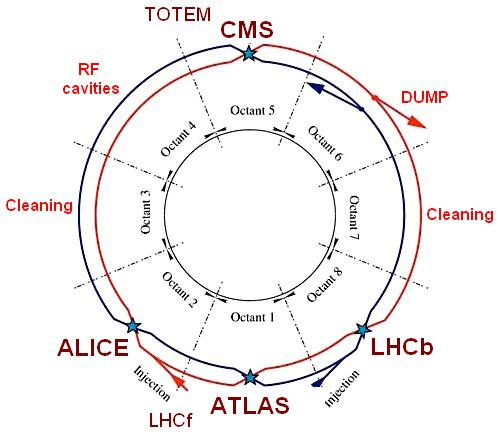
\includegraphics{figuras/Chapter2/LHCrings}}
\caption{Schematic view of the LHC proton rings with the interaction points, 
where the CMS, ATLAS, ALICE and LHCb detectors are located.}\label{chp2:LHCringsfigure}
\end{center}
\end{figure}

\subsection{Pronton Accelerator Chain}
\label{subsec:ProtonAcceleratorChain}

%at an energy of 450 GeV, they have several

Before bunches of protons are injected into the two LHC rings, also known as LHC main ring, they have several
pre-acceleration stages  shown in Figure \ref{chp2:LHCaccelerationchain}. The process starts with the extraction of protons 
in the Duoplasmatron Proton Ion Source. In the proton source, the protons are extracted by
ionization of Hydrogen gas. As result, bunches of protons are injected into a linear 
accelerator, Linac2, where their energy is increased up to 50 MeV. Once the protons 
reach such energy, they are delivered to the Proton Synchrotron Booster (PSB) and then to the
Proton Synchrotron (PS) where they are accelerated up to 1.4 GeV and 25 GeV, respectively. Additionally,
in the PS the bunches of protons are splitted into bunches spaced by 
25 ns\footnote{For the Run I, the bunches were spaced by 50 ns}. Finally, 
the pre-acceleration chain finishes in the Super Proton Synchrotron (SPS), where 
the protons reach an energy up to 450 GeV before they are injected into the LHC rings. The 
protons are injected into the LHC rings in opposite directions, clockwise and counter-clockwise, where 
they can reach an energy up to 7 TeV.

\begin{figure}[ht]
\begin{center}
 \scalebox{0.3}{
          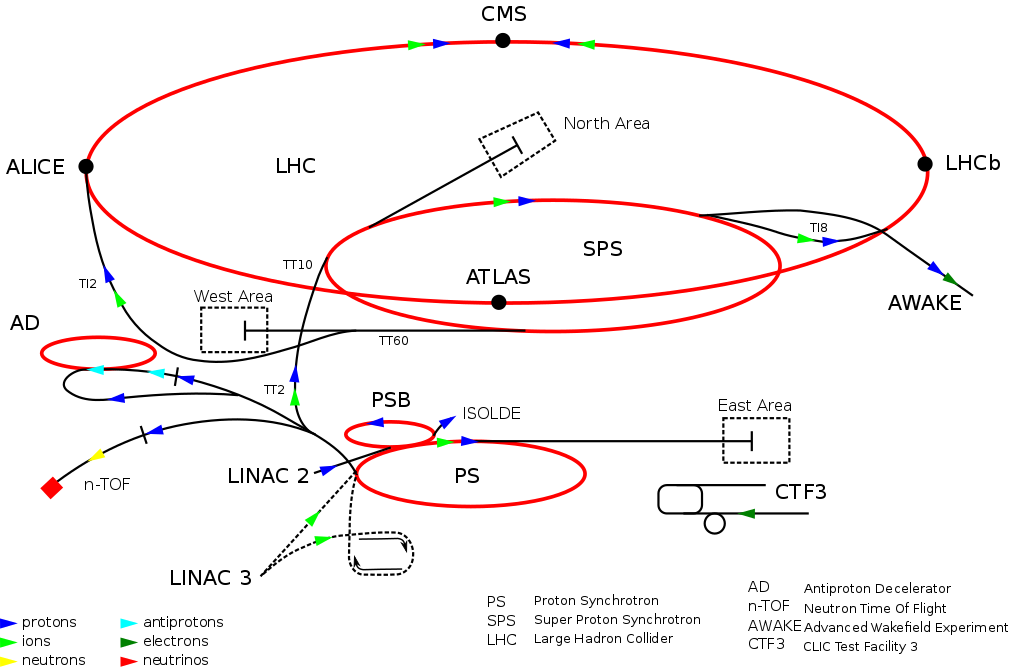
\includegraphics{figuras/Chapter2/LHCaccelerationchain2}}
\caption{Schematic view of the proton accelerator chain at CERN.}\label{chp2:LHCaccelerationchain}
\end{center}
\end{figure}


\subsection{LHC ring}
\label{subsec:LHCring}



\section{The CMS Detector}
\label{sec:CMS}

\section{The Tracker System}
\label{sec:Tracker}

\subsection{Pixel Tracker}
\label{subsec:Pixel}

\subsection{Silicon Strip Detector}
\label{subsec:Strip}

\section{Electromagnetic Calorimeter}
\label{sec:ECal}

\section{Hadronic Calorimeter}
\label{sec:HCal}

\section{Muon System}
\label{sec:MuonSys}

\subsection{RPCs}
\label{subsec:RPCs}

\subsection{DTs}
\label{subsec:DTs}

\subsection{CSCs}
\label{subsec:CSCs}

\subsection{GEMs}
\label{subsec:GEMs}

\section{Particle Reconstruction}
\label{sec:ParticleReconstruction}

\subsection{Trigger}
\label{subsec:Trigger}

\subsection{Data Adquisition}
\label{subsec:DAQ}

\subsection{Physics Objects}
\label{subsec:PhysicsObjects}


%Tau Leptons
\chapter[Particle Identification and Event Reconstruction]{Particle Identification and Event Reconstruction}
\label{chap:ParticleID}




\section{Particle Flow}
\label{sec:PF}

The Particle Flow (PF) algorithm \cite{CMS-PAS-PFT-09-001} identifies and reconstructs all the stable-visible particles produced in the hard interaction, by
combining the information collected by the CMS sub-detectors in order to optimize the determination of their direction, energy and type. The PF 
technique performs the global event reconstruction classifying all the visible particles into five mutually exclusive groups: photons, 
neutral hadrons, charged hadrons, electrons and muons. This list of individual particles (called ``PF Candidates'') are used 
as an input in further algorithms to reconstruct higher level objects such as jets, missing transverse energy and tau-leptons. \\

%The capabilities of the CMS detector are ideal for using the PF technique as a global event reconstruction. The high 
%granularity of the inner tracker and the ECAL, the hermiticity of the HCAL, the high performance of the muon system 
%along with the strong magnetic field provided by the superconducting solenoid allow PF technique to reach a 
%high performance reconstruction for the individual particles produced in the hard interaction, even for charged particles
%with very low $\textrm{p}_{\textrm{T}}$ of an order of 100 MeV; this leads to an improvement in the energy jet corrections. Besides, the high performance of the individual particle reconstruction 
%allows to discriminate between nearby tracks such as the decay products of the tau-lepton. The main advantage 
%to use the PF technique as a global event reconstruction is the high performance reconstruction 
%for all the physics objects, in particular jets, MET and tau-leptons \cite{CMS-PAS-PFT-10-001}.\\


The capabilities of the CMS detector are ideal for using the PF technique as a global event reconstruction. The high 
granularity of the inner tracker and the ECAL, the hermiticity of the HCAL, the high performance of the muon system 
along with the strong magnetic field provided by the superconducting solenoid allow PF technique to reach a 
high performance reconstruction for the individual particles produced in the hard interaction, even for charged particles
with very low $\textrm{p}_{\textrm{T}}$ (of the order of 100 MeV). This leads to an improvement in the global event 
reconstruction since, instead of using special sub-detectors designed to reconstruct an specific 
object (like alternative event reconstruction techniques), PF algorithm uses a more completed information collected 
by all CMS sub-detectors, avoiding any ambiguity to reconstruct the object. Besides, the 
individual particle reconstruction provides a detailed information 
about compositeness of high level objects like jets, allowing PF technique
to determinate the hadron profile of the jet and its origin, which is important for the tau-identification. 
Additionally, the high performance of individual particle reconstruction allows to discriminate between nearby tracks 
such as the decay products of the tau-lepton. The main advantage 
to use the PF technique as a global event reconstruction is the high performance reconstruction 
for all the physics objects, in particular jets, MET and tau-leptons \cite{CMS-PAS-PFT-10-001}.\\

%and the ECAL, the hermicity of the HCand clusters with high efficiency.

The PF technique is performed in three steps: First, the algorithm builds the so-called ``PF elements'' which consist of tracks 
reconstructed in the Inner Tracker, energy clusters reconstructed in the calorimeters and tracks observed in the muon system;
the second stage addresses the topological association of the basic PF elements each other using the ``link-algorithm''; finally,
individual particles are identified and reconstructed from the content of the linked elements. \\

%Photons are reconstructed from its energy deposits in the ECAL (See section \ref{sec:Photon});
%electrons are reconstructed by the combination of tracks and the energy deposits in the ECAL of the electron itself and the 
%Brestrahlung radiation produced by its interaction with the tracker material (See section \ref{sec:Electron}); Muon reconstruction 
%is performed connecting together the tracks reconstructed by the inner tracker and the muon system, it will be described in section \ref{sec:Muon};

\subsection{Track Reconstruction}
\label{subsec:TrackReco}
The track reconstruction in the inner tracker is one of the most important keys of the global event reconstruction. The inner tracker, due to its
high granularity, provides a precise reconstruction of the charged-particle tracks and consequently give rise to an accurate reconstruction 
of the primary vertex, identifying it from the pileup interactions. \\

The track reconstruction is performed in several steps by a process called \textit{iterative tracking}. In the initial iterations, 
the iterative tracking applies a tight criteria in order to search for tracks easy to identify (tracks 
with relative high $\textrm{p}_{\textrm{T}}$ produced near the interaction region). In the next iterations, the hits 
unambiguously assigned to a track are removed. This reduces the combinatorial complexity in the subsequent iterations 
and allows to loosen the selection criteria to identify the tracks associated with low $\textrm{p}_{\textrm{T}}$. In the first three iterations, 
the iterative tracking reaches an efficiency up to 99.5$\%$ for isolated muons and larger than 90$\%$ for 
charged hadrons in jets \cite{CMS-PAS-PFT-09-001}. Last iterations relaxes the constrains on the origin of the vertex 
to find tracks originated outside the beam spot (secondary charged particles from photon conversions in the tracker material) 
and to reconstruct the remaining tracks. Each iteration could be summarized in 4 steps:\\

\begin{itemize}
 \item Tracks are seeded using 2 or 3 hits, giving rise to the initial track candidates and their initial trajectory parameters.
 \item The track finder algorithm is based on the Kalman filter \cite{Fruhwirth:1987fm}, which consist in an extrapolation outwards of the inner 
       tracker layers with the purpose to find additional hits associated to the track and to estimate the track 
       parameters. The filter recalculates the track parameters for each layer, accounting the energy loss and the 
       multiple Coulomb scattering produced by the interaction of the charged particle and the tracker material.
 \item A fit on the track is performed to estimate all the possible information of the trajectory.
 \item Tracks are selected on basis of the quality flags, whether they are compatible with some 
 criteria such as $\chi^{2}$ and if they are originated from the primary vertex.
\end{itemize}

The efficiency estimation of the track reconstruction is performed comparing the reconstructed tracks with MC samples which 
contains just single muons or pions. Muons are ideal for this purpose since muons, unlike electrons, have a negligible energy loss
through bremsstrahlung radiation due to the interaction with the tracker material. Unlike muons, charged pions (a tau decay product) do not 
only undergo Coulomb scattering but it (as all hadrons) also loses energy though strong interactions with the tracker material. These nuclear 
interactions are not taken into account in the track Finder algorithm, reducing the track reconstruction efficiency. The tracking efficiency 
is higher than 99$\%$ for isolated muons with a $\textrm{p}_{\textrm{T}}>1$ $\textrm{GeV}$ while for charged pions is close 
to 95$\%$ for $\textrm{p}_{\textrm{T}}>1$ $\textrm{GeV}$ \footnote{Efficiencies were obtained from 2011 data for pp collision  
at a centre-of-mass energy of $\sqrt{s} =$  7 TeV. For simulated events an average of 8 for pileup interactions was used, which corresponds
roughly to the amount delivered by the LHC on 2011.} \cite{Chatrchyan:2014fea} (See Figure \ref{fig:Track_Efficiencies}). The PU interactions
degrades significantly the tracking efficiency for tracks with $\textrm{p}_{\textrm{T}}<1$ $\textrm{GeV}$ \cite{Chatrchyan:2014fea}


%The tracking
%efficiency depends, besides on the $\textrm{p}_{\textrm{T}}$, on $\eta$ due the geometrical acceptance of the tracker and 
%the PU which degrades the efficiency for tracks with $\textrm{p}_{\textrm{T}}<1$ $\textrm{GeV}$




\begin{figure}[ht]
  \begin{center}
    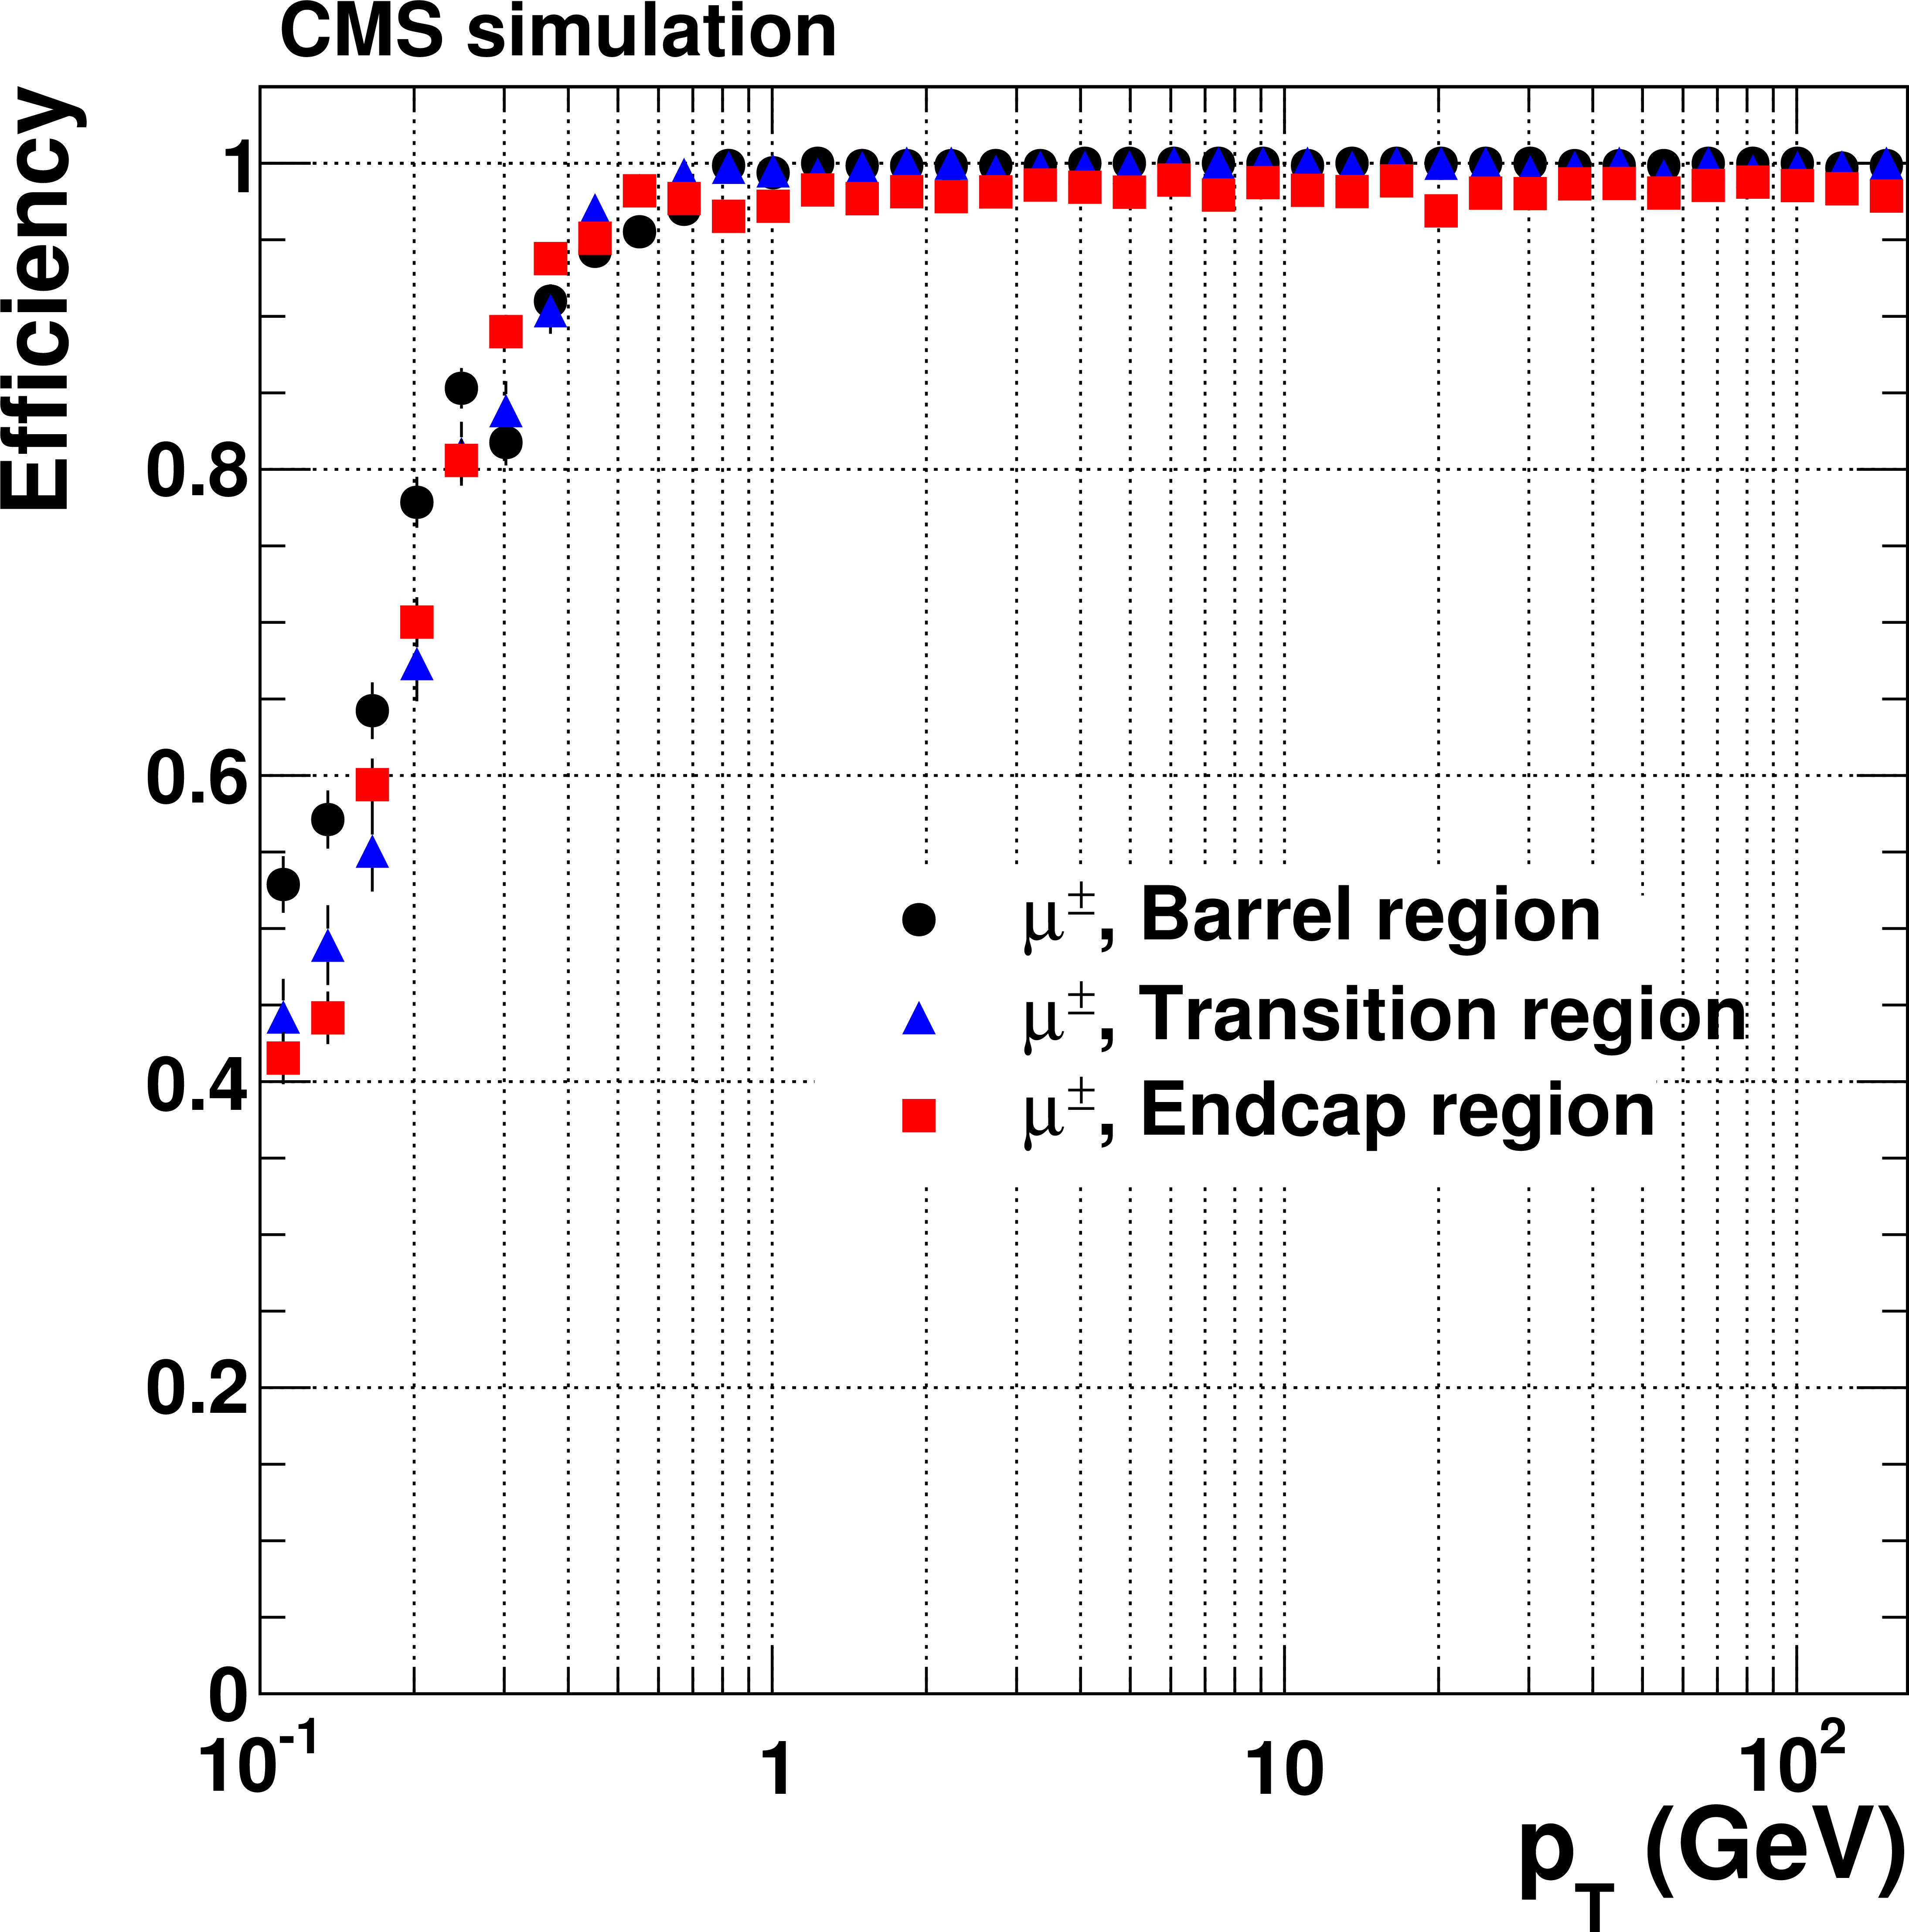
\includegraphics[width=0.35\textwidth]{figuras/Chapter3/TrackEff_Muon_pt.png}
    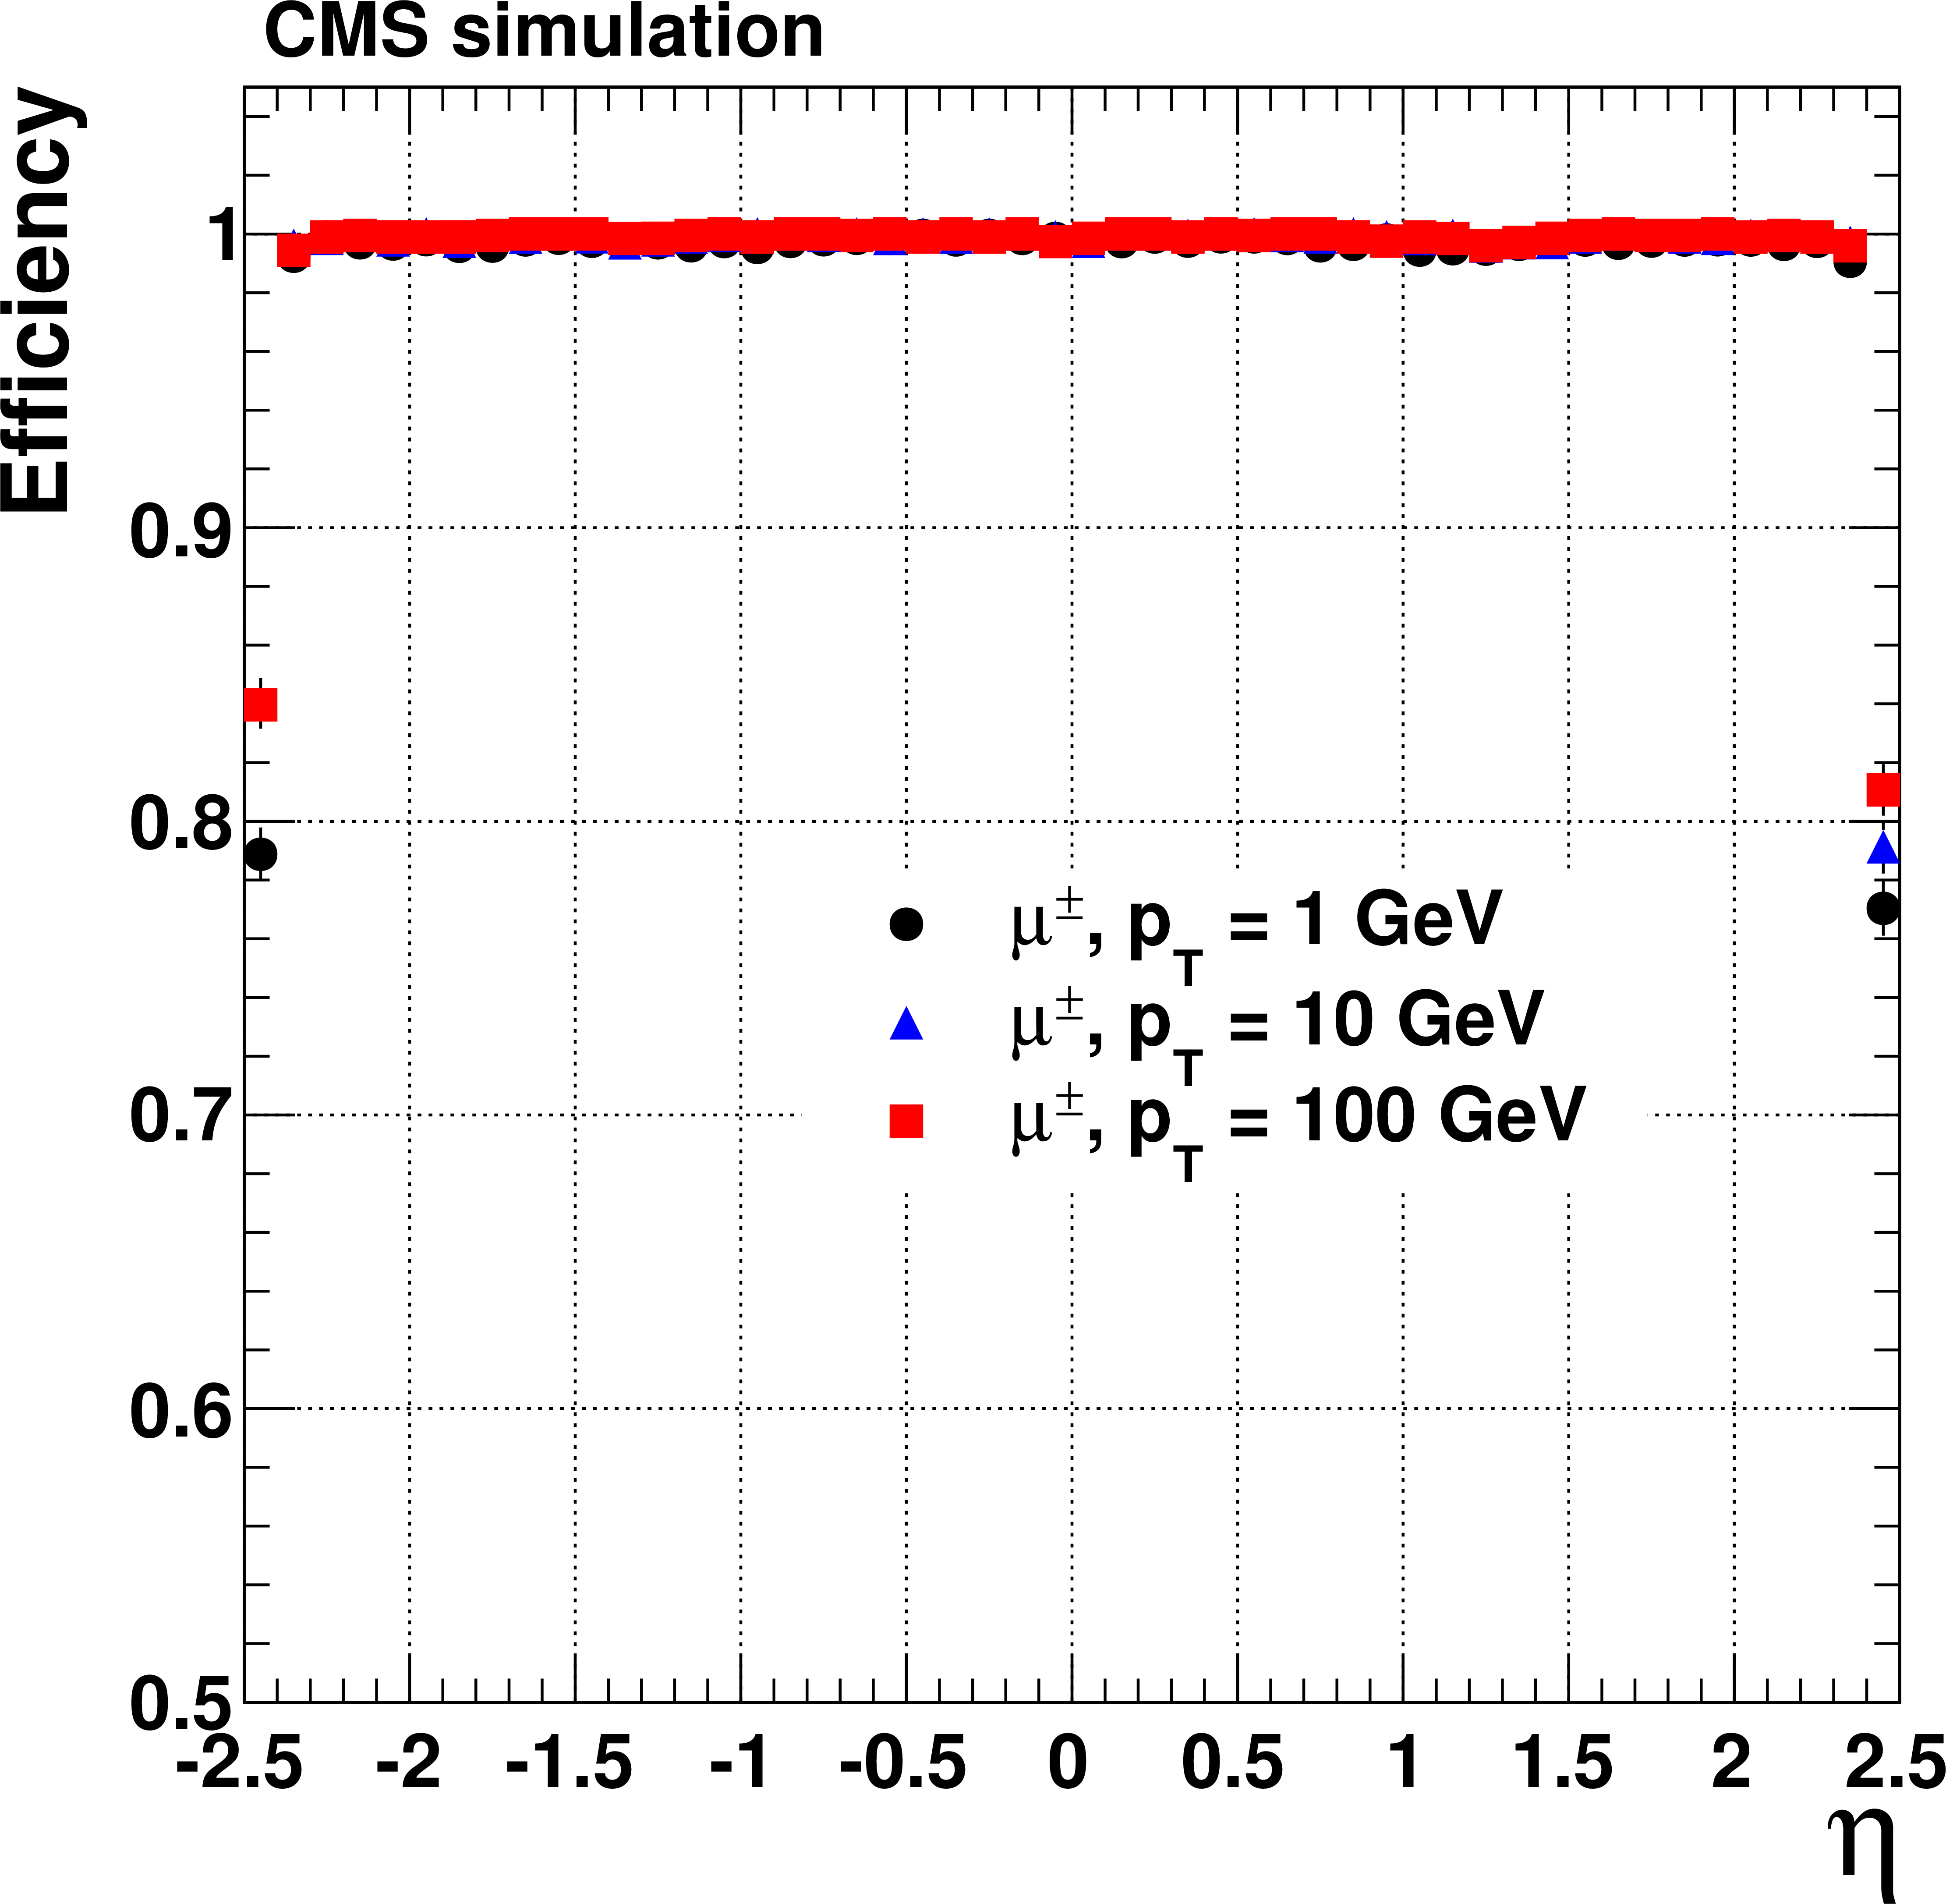
\includegraphics[width=0.35\textwidth]{figuras/Chapter3/TrackEff_Muon_eta.png}
    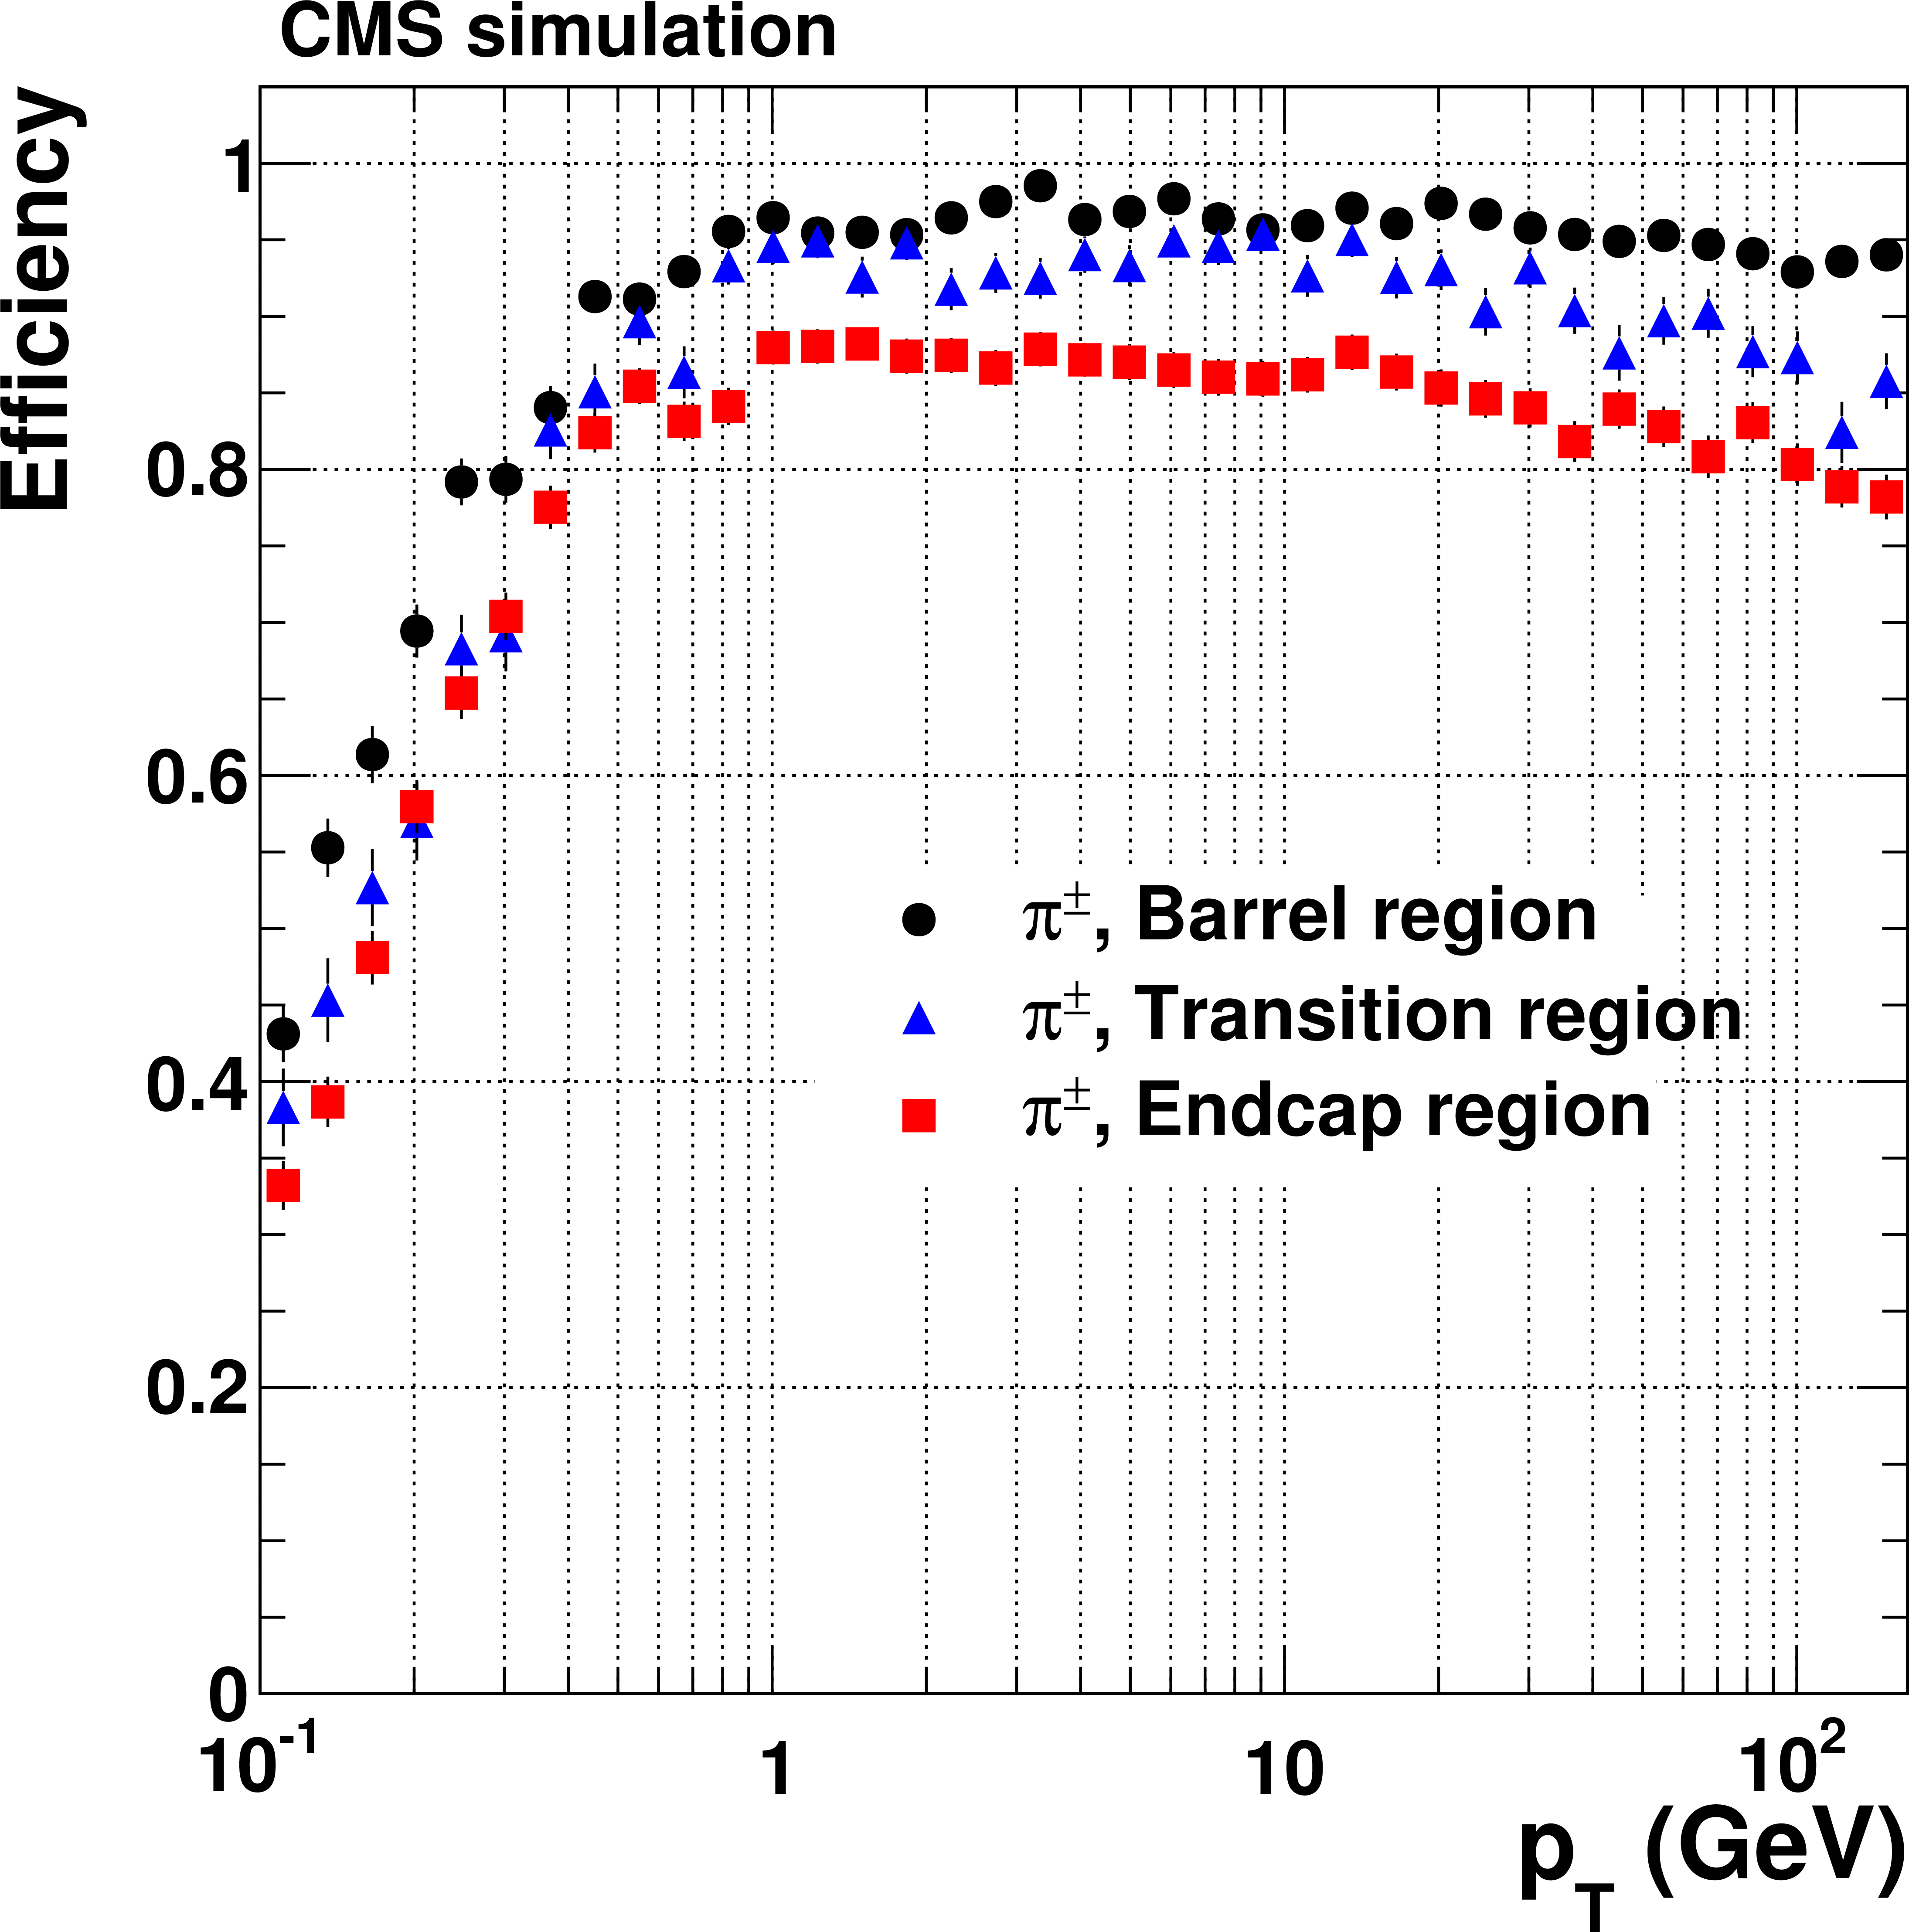
\includegraphics[width=0.35\textwidth]{figuras/Chapter3/TrackEff_Pion_pt.png}
    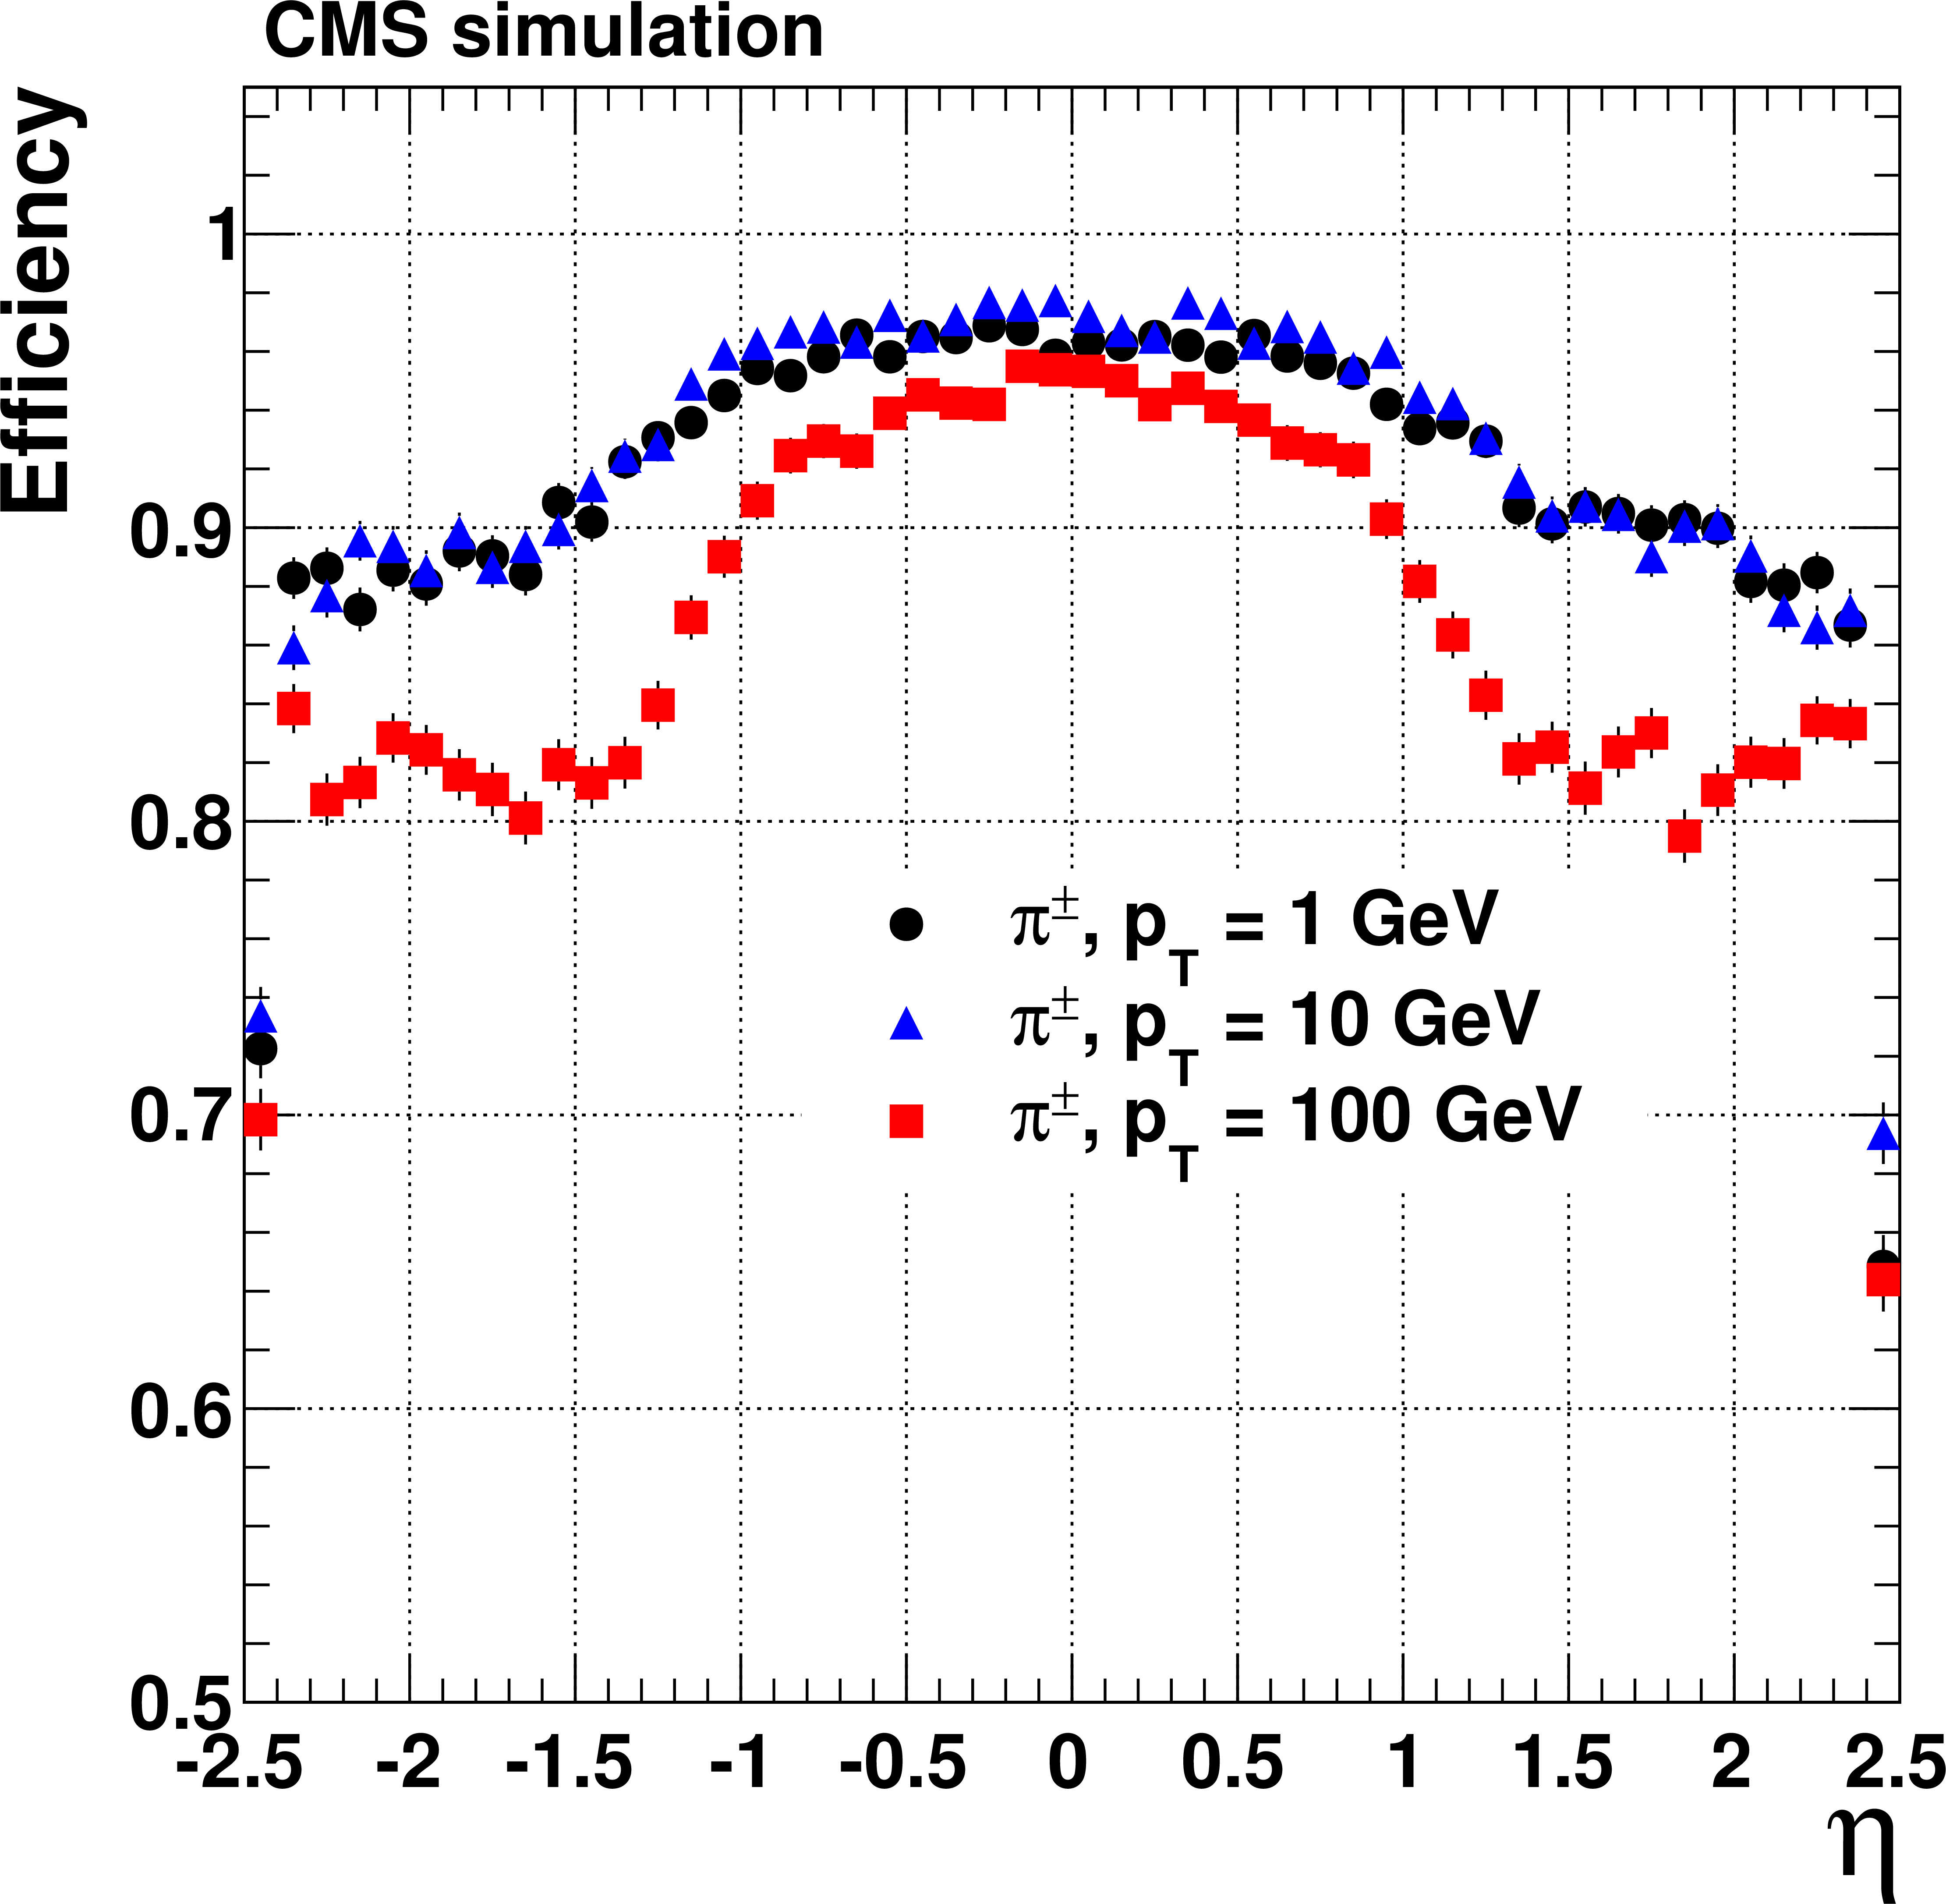
\includegraphics[width=0.35\textwidth]{figuras/Chapter3/TrackEff_Pion_eta.png}
    \caption{Efficiency of reconstructed track as function of $p_{\textrm{T}}$ and $\eta$ for 
    muons (top) and charged pions (bottom). Efficiencies were obtained using pp collisions with a centre-of-mass 
    energy of $\sqrt{s} =$  7 TeV, which corresponds to 2011 data. For simulated data an average of 8 pileup 
    events was used, which is roughly the amount delivered by the LHC on 2011. Figure taken from \cite{Chatrchyan:2014fea}}
    \label{fig:Track_Efficiencies}
  \end{center}
\end{figure}

\subsection{Vertex Reconstruction}

%Primary vertex reconstruction is performed with the purpose to measure the position, and the uncertainty, 
%of all vertices produced in the pp collisions, such as the vertex produced by a hard interaction, secondary 
%vertices coming from b-jets as well as pileup collisions. Vertex reconstruction first proceed with a 
%track selection, then reconstructed tracks are clustered to identify vertices, and finally the vertex position
%is determined by a fit. \\

Primary vertex reconstruction is performed with the purpose to measure the position, and the uncertainty, 
of all vertices produced in the pp collisions. Vertex reconstruction first proceed with a 
track selection, then reconstructed tracks are clustered to identify vertices, and finally the vertex position
is determined by a fit. The main criteria for track selection are the impact parameter relative to the beam spot, the
number of reconstructed hits in the tracker and the $\chi^{2}$ associated to its trajectory. Then, the 
selected tracks are grouped into clusters according to its z-coordinate with the aim of identifying
all possible vertices even for inelastic collisions. Track clustering is performed with the 
deterministic annealing (DA) algorithm \cite{VertexRecoBIB}. The DA algorithm resolves iteratively
the z-coordinates of all the possible vertices and the cluster of tracks associated to them, in a similar way 
to solve a physical system with many degrees of freedom, approaching iteratively to the state 
of minimum energy \cite{Chatrchyan:2014fea}. Finally, the adaptive vertex fitter technique \cite{Frühwirth:1027031}
is used in order to perform the best estimation of the vertex parameters, in particular the position,
from fitting the cluster of tracks associated to the vertex. The primary vertex is selected from the vertex with the higher
sum of $\textrm{p}_{\textrm{T}}^{2}$ of the cluster of tracks.\\

The resolution of the primary vertex depends on the number of tracks associated to it. Figure \ref{fig:RecoVertex} 
shows the resolution of x and z position for primary vertex reconstruction, using minimum vias samples 
\footnote{minimum vias samples pass a suit of triggers and minimum requirements on hit 
or track multiplicity} and jet-enriched data samples \cite{Chatrchyan:2014fea}. The resolution for x and z position 
is, respectively, less than 20 $\mu$m and 25 $\mu$m for the minimum vias samples while it is 
improved to less than 10 $\mu$m and 12 $\mu$m for jet-enriched samples. Figure \ref{fig:RecoVertex} c) shows
the efficiency of primary-vertex reconstruction which depends on the number of tracks. 

\begin{figure}[ht]
  \begin{center}
    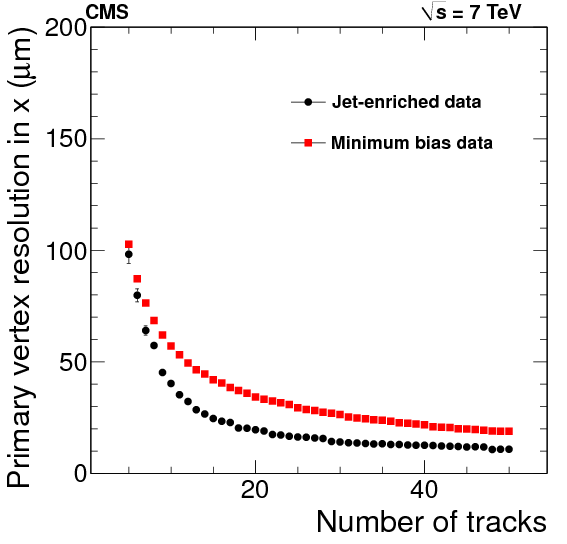
\includegraphics[width=0.3\textwidth]{figuras/Chapter3/RecoVertex_x_resolution.png}
    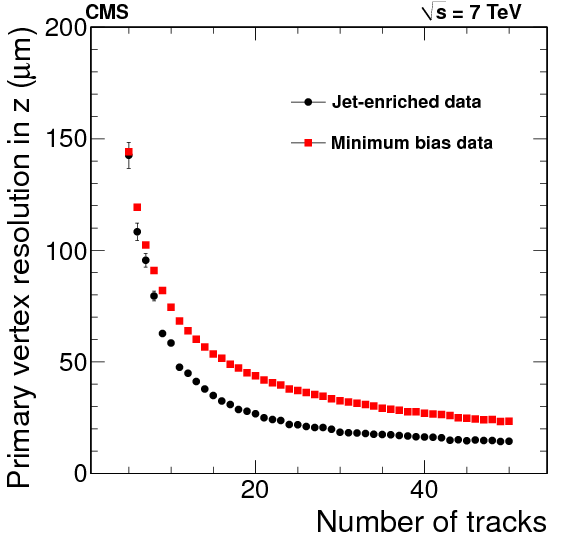
\includegraphics[width=0.3\textwidth]{figuras/Chapter3/RecoVertex_y_resolution.png}
    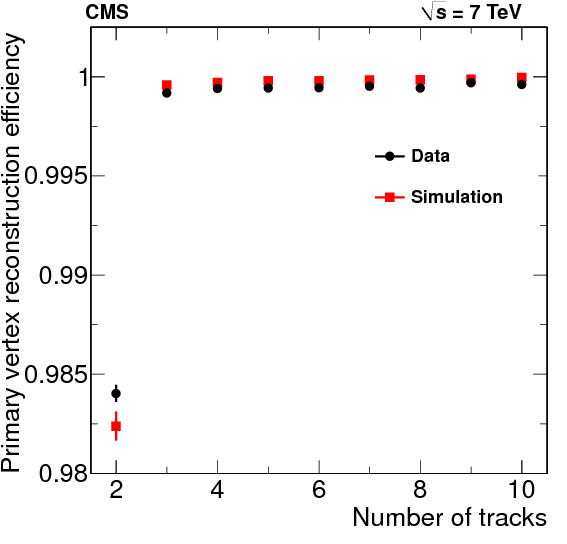
\includegraphics[width=0.3\textwidth]{figuras/Chapter3/Effciiency_vertex_resolution.png}
    \caption{Resolution of x and z position  for primary vertex reconstruction, using a) minimum vias samples and b) jet-enriched samples. 
    Resolution is improved using jet-enriched samples since in these sample the mean of $\textrm{p}_{\textrm{T}}$ is larger than minimum vias samples.  
    For efficiency of primary vertex reconstruction shown in c), minimum vias MC samples were used. Results were estimated 
    with pp collisions with a centre-of-mass energy of $\sqrt{s} =$  7 TeV. Figures were taken from \cite{Chatrchyan:2014fea}.}
    \label{fig:RecoVertex}
  \end{center}
\end{figure}

%El algoritmo lo que hace es buscar la minima temperatura ``T'' local para el cual chi2 sea minima, 
% comienza con T-> inf, todos los tracks estan asociados a un solo vertice, la T comienza a disminuir,
% comienza a crecer el numero de vertices, se hace eso hasta que el sistema alcanza la Tcritica (el punto de inflexion de la energia libre F)
% (chi2 hace las veces de la eneria)
% una vez se encuentra el minimo local, cada vertice se convierte en dos, endonde el peso asociados a esos vertices es igual al vertice ``papa''
% eso se hace iterativamente hasta alcanzar una T igual a 4 en donde ya hay una posibilidad de convertir un real vertice en dos.


\subsection{Clustering}
\label{subsec:Clustering}
Other important part of the PF technique, in addition to the tracks, is the reconstruction of the 
calorimetric clusters. The calorimeter clusters are used to identify the energy deposits which come from 
%neutral-visible particles, such as photons and neutral hadrons, and discriminate them from the energy deposits 
photons and neutral hadrons, and to discriminate them from the energy deposits due charged hadrons; 
besides it reconstructs the electrons along with their associated Bremsstrahlung radiation
and helps to determinate the track parameters of the charged hadrons which were not measured 
accurately from the track reconstruction (for example, charged hadrons that are outside of the tracker acceptance, or 
charged hadrons with high $p_{\textrm{T}}$). The clustering is performed for 
each part of the CMS calorimeter system: ECAL, HCAL, HF and PS.\\

The clustering algorithm proceeds from the ``cluster seeds'' identified at local level. Cluster seeds are selected 
from individual calorimeter cells which have a maximal energy deposits above a given energy. Once the cluster seed is selected,
the algorithm searches for energy deposits in the  boundary cells with a common side. The algorithm aggregates to the cluster 
at least one additional cell with a maximum energy higher than two standard deviations from the electronic noise: for the ECAL, 80 $\textrm{MeV}$ in 
barrel and up to 300 $\textrm{MeV}$ in the end-caps for the ECAL, while 800 $\textrm{MeV}$ for the HCAL \cite{CMS-PAS-PFT-09-001}. This
cells combined are known as ``topological clusters''. The topological clusters are taken as ``particle flow clusters'' seeds
in order to solve any overlapping among clusters.

\subsection{Link algorithm}
\label{subsec:Linkalgorithm}
As mentioned earlier, a particle is expected to produce signatures in different sub-detectors, giving rise to one or more 
so-called PF elements: tracks, clusters and tracks in the muon system; for example, 
a charged hadron as the pion, would produce a track in the inner tracker along with 
energy deposits in both calorimeters. PF uses the \textit{link algorithm} to perform a topological combination 
of the PF elements reconstructed in the different sub-detectors with the aim of reconstructing fully each particle in the event. \\
%of the PF elements recontructed in the different subdetectors with the aim of identifying the type of each particle in the event. 

The link between a charged particle track and a calorimeter cluster is performed as follows:

\begin{itemize}
 \item The track is extrapolated from the last hit reconstructed in the tracker to: the two layers in the PS, the expected depth
 for an electron shower in the ECAL and one interaction length for an typical hadron shower in the HCAL. 
 \item The track is linked to a cluster if the extrapolated position in the calorimeter is within the cluster boundaries. 
 \item The distance in the $\eta-\phi$ plane between the extrapolated track position and the cluster position defines the quality of the link. 
\end{itemize}

Similarly, two calorimeter clusters (i.e. links between PS and ECAL clusters or links between ECAL and HCAL clusters) are linked when the 
extrapolated position in the more granular calorimeter (PS or ECAL) is within 
the boundaries of the less granular calorimeter (ECAL or HCAL). For example, the link between the ECAL and HCAL clusters
produced by a pion is established when the extrapolated position from the ECAL is within the HCAL cluster boundary. Finally, the 
link between a charged particle track reconstructed in the tracker and a track in the muon system (known as global muon) 
is established by a global fit between the two tracks and its $\chi^{2}$ defines the quality of the link.  

\section{Jets Reconstruction}
\label{sec:Jet}


% Jets are reconstructed with the Particle Flow technique (PF) using the anti$-$k$_{T}$ algorithm \cite{Alwall:2011uj}.
The PF technique \cite{CMS-PAS-PFT-09-001} takes the information collected by the CMS sub-detectors in order to identify and reconstruct
all the visible final-state particles (electrons, muons, photons, charged hadrons and neutral hadrons) produced
in the hard interaction. The PF technique reconstructs the jet constituents individually from the
combination of tracks and calorimeter clusters. Then, the jet reconstruction is performed
with the anti$-$k$_{T}$ algorithm \cite{AntiKTAlgorithm} iterating over all the PF objects, using a distance parameter of
$\Delta R = 0.4$ in the $\eta-\phi$ plane, where $\Delta R = \sqrt{(\Delta \phi)^2+(\Delta \eta)^2}$.\\

\begin{figure}[ht]%[!Hhtbp]
  \begin{center}
    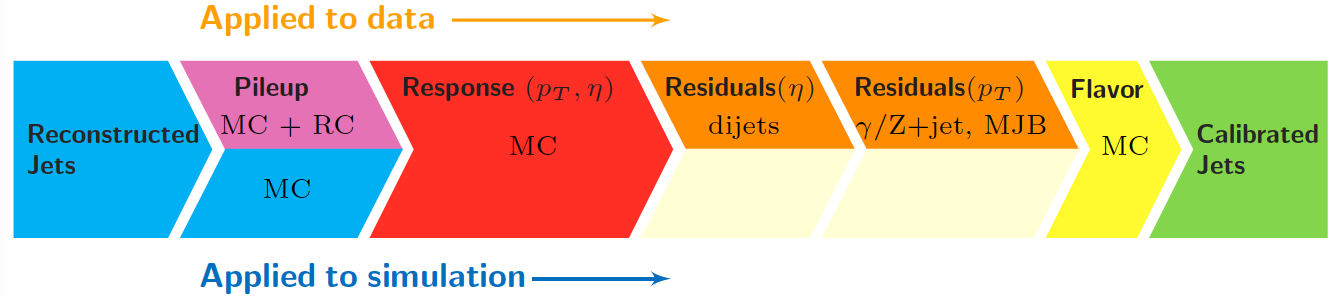
\includegraphics[width=0.9\textwidth]{figuras/Chapter3/JEC_levels.png}
    \caption{Levels of corrections for PF jet four-momentum. Figure taken from \cite{JESandJER}}
    \label{fig:JEC_levels}
  \end{center}
\end{figure}

The four-momentum of the reconstructed jet is the addition of the four-momenta of all the PF objects associated to the jet. However
due to detector responses and experimental effects, the PF jet four-momentum does not correspond to the four-momentum
at parton or hadron level; therefore, jet energy corrections (JEC) are required. Figure \ref{fig:JEC_levels} shows the different
levels of corrections which are applied in a fixed sequence. Each correction corresponds to a multiplicative factor $C$ on
the PF jet four-momentum ($p_{\mu}^{raw}$):

\begin{equation}
 p_{\mu}^{corrected} = C \times p_{\mu}^{raw}
\end{equation}

The first step in the chain is the ``L1 corrections'' (also referred as ``pileup offset''). It corrects the additional tracks and the excess of energy deposits
in the calorimeters due pile-up events . The amount of the pile-up contribution
to the jet energy can be estimated from the global per-event $p_{T,offset}$ density $\rho$ and the jet area \cite{JECpileup}. This amount
is obtained from simulated dijet events with and without PU. \\

The second level of JEC is related to the detector response to hadrons (L2L3 MC-truth corrections), correcting
the non-uniformity in $\eta$ and the non-linearity in $p_{T}$. The simulated jet response is determined
with QCD-multijet events generated with Pythia and with a simulation of the CMS detector based
on Geant4.\\

After these steps, the L2L3 Residual corrections are applied in order to address the remaining difference
between the jet response on data and MC (of the order of $1 \%$). This corrections are achieved with data-driven methods, using
dijet samples for $\eta$-dependent corrections and $\gamma /$Z+jets samples for the corrections to $p_{T}$. The last stage
of the JEC (L5) is optional and it accounts the jet-flavor corrections. \\

%An efficiency larger than 80% is obtained for jets with a p T > 20 GeV/c. The 100% plateau is reached above
%40 GeV/c, at which point the mismatched jet rate is negligible





%JER Article
%The jet p T resolutions are determined with both dijet and photon+jet events, as discussed in
%section 8. The reference resolutions obtained from simulation are parameterized as a function of
%particle-level jet p T, ptcl (defined in section 2) and average number μ of pileup interactions in bins
%of jet η. Corrections for differences between data and MC simulation are applied as η-binned scale
%factors




%Since in average 85 $\%$ of the constituents of a jet are charged particles and photons, the jet energy resolution

%PF jet momentum and spatial resolutions are greatly improved with respect to calorimeter jets, as
%the use of the tracking detectors and high granularity of the ECAL improves the energy resolution
%through the independent measurements of charged hadrons and photons inside a jet, which together
%2.1constitute ≈85% of the average jet energy. In reconstructing the PF candidate four-momentum,
%photons are assumed massless and charged hadrons are assigned the charged pion mass.

%As mentioned previously, the typical jet energy fractions carried by charged particles, photons
%and neutral hadrons are 65%, 25% and 10% respectively. These fractions ensure that 90% of
%the jet energy can be reconstructed with good precision by the particle-flow algorithm, both in
%value and direction, while only 10% of the energy is affected by the poor hadron calorimeter
%resolution and by calibration corrections of the order of 10 to 20%. As a natural consequence,
%it is expected that jets made of reconstructed particles be much closer to jets made of MonteCarlo–generated
%particles than jets made from the sole calorimeter information, in energy, direction
%and content. It is the purpose of this section to quantify this statement.

%($c\tau > 1$ cm)


%\subsection{Online Identification}
%\label{subsec:JetTrigger}

%\subsection{Offline Identification}
%\label{subsec:JetReconstruction}



%\subsection{Online Identification}
%\label{subsec:ElectronTrigger}

%\subsection{Offline Identification}
%\label{subsec:ElectronReconstruction}
\section{MET}
\label{sec:MET}

\section{Photon Reconstruction}
\label{sec:Photon}


\section{Muon Reconstruction}
\label{sec:Muon}

\section{Electron Reconstruction}
\label{sec:Electron}

\section{B-Jet Reconstruction}
\label{sec:BJet}



\section{Tau Lepton}
\label{sec:Tau}

%\subsection{Tau Reconstruction}
%\label{subsec:TauTrigger}

\subsection{Tau Reconstruction}
\label{subsec:TauReconstruction}

\subsection{Working Points}
\label{subsec:wp}

\subsubsection{Efficiency of Working Points}
\label{subsubsec:Eff_WP}

\subsection{Fake Rates}
\label{subsec:FakeRates}

\subsection{Perspectives Run III}
\label{subsec:Perspectives} 

%High Mass resonances decaying into tau leptons.
%\chapter[MC event generation]{Monte-Carlo event simulation}
\label{chap:MC}


\section{Monte-Carlo simulations}
\label{sec:MC}


%Analysis chapter
\chapter[Search For \Zprime~Bosons With 2016 Data]{Search for \Zprime~Bosons with 2016 Data}
\label{chap:Analysis}

\section{Analysis Strategy}
\label{sec:Strategy}

\section{Data sets and Monte Carlo samples}
\label{sec:Samples}

\section{Trigger}
\label{sec:Trigger}

\subsection{Trigger Efficiency}
\label{subsec:TriggerEff}

\section{Event Selection}
\label{sec:EventSelection}

\section{Background Estimation}
\label{sec:BackgroundEstimation}

\subsection{QCD}
\label{subsec:QCD}

\subsection{Drell-Yan}
\label{subsec:QDY}

\section{Systematics}
\label{sec:Systematics}

\section{Results}
\label{sec:Results}


%Conclusions
%\chapter*{Conclusions}
\chapter[Conclusions]{Conclusions}
\label{chap:Conclusions}

Conclusions



%Appepdices
%\appendix
%\include{DataDriven}
%\chapter{Signal modeling}
\label{chap:sigmod}

In chapter \ref{chap:SM} of this work, the different possibilities of VLQ models implementations have been discussed. For the analysis presented in chapter~\ref{chap:search}, a specific model of VLQ's have been used for the MC simulations of a vector like \Tp. However, different models can be also studied, as shown in table~\ref{tab:VLQRepre}. Their predictions are similar, but the objects kinematics can be in principle different for the same production channel. The purpose of this appendix is to look in detail, at generator level, the kinematics of \Tp~and the associated jet in the single production mode for the different models. %With such study an estimation of the observability of the \Tp~with different models is done. %, the possibilities of the presented analysis to see a similar object to the one considered.

\section{Model Independence}
\label{sec:modindp}

There are three different possibilities to have a vector like \Tp, either as a singlet or as a member of a standard doublet ($Y=7/6$) or a non-standard doublet ($Y=1/6$). On the following, the singlet will be noted as T, the standard doublet as TB and the non-standard doublet as XT. The vector like \Tp~can be mixed to third or light generations of SM quarks exclusively, or can be mixed to the three generations. For the single production mode only the singlet representation can be mixed exclusively to third generation. The doublets should be mixed to the three generations or exclusively to light generations. These mixings are controlled by one single parameter for the MC generation, $R_{L}$. A $R_{L}=0$ stands for exclusive mixing to third generation, $R_{L}=\infty$ for exclusive mixing to light generations and $R_{L}=0.5$ for shared mixings to all three SM quark generations. 

On the plots that will be presented, the convention for the legend is \textit{Representation\_ $R_{L}$ value \_ Production channel}. For example, XT\_RLInf\_Tj stands for the XT doublet representation with $R_{L}=\infty$ in the single production of a vector like \Tp~associated to a jet. Figure~\ref{fig:accomjet} shows the distributions for the \pt~and $\eta$ of the jet produced in association with the \Tp~in the single production mode for all possible models and mixings. The comparison is performed with MC samples for a mass of the \Tp~of 700 \GeVcc, at parton level. No significant differences between models or mixings is observed for the majority of cases. However, the case of the singlet with exclusive mixing to third SM quark generation presents a more forward $\eta$ for the jet produced with the \Tp. Figure~\ref{fig:Tppt} displays the comparison between different models of the \pt~of \Tp. 

\begin{figure}[!hbtp]
  \begin{center}
    \includegraphics[width=0.45\textwidth]{figs/Ana/eta6thjetmodels.png}
    \includegraphics[width=0.45\textwidth]{figs/Ana/pt6thjetmodels.png}
    \caption{$\eta$ and $p_{T}$ of the associated jet produced with the \Tp~for different representations and couplings with SM quarks. The case of the singlet with exclusive mixing to third generation (T\_RL0\_Tj) produce a more forward associated jet than the rest of models.}
    \label{fig:accomjet}
  \end{center}
\end{figure}

\begin{figure}[!hbtp]
  \begin{center}
    \includegraphics[width=0.5\textwidth]{figs/Ana/ptTpmodels.png}
    \caption{$p_{T}$ of the \Tp~for different representations and couplings with SM quarks}
    \label{fig:Tppt}
  \end{center}
\end{figure}

In addition, as in the selection there is a cut on the $\Delta R$ between \Tp~and the associated jet, the distribution for this variable for different models can be found in figure~\ref{fig:DRmodels}. In this variable also no significant differences are seen between the majority of models. In this variable also the T\_RL0\_Tj case differs from others. The differences between the models should be diminished when considering hadronization and showering of MC samples.

\begin{figure}[!hbtp]
  \begin{center}
    \includegraphics[width=0.5\textwidth]{figs/Ana/DRmodels.png}
    \caption{$\Delta R (Tj)$ for different representations and couplings with SM quarks}
    \label{fig:DRmodels}
  \end{center}
\end{figure}

%We consider then as maximum a 5\% systematic uncertainty from differences shown between possible models, to take into account the theoretical predictions of kinematics of \Tp~and the associated jet in the single production mode.

\section{\Tjj~compared to \Tj}

The cross sections used as theoretical prediction were obtained considering only the main production process of \Tp~with only one associated jet. However, if the vector like \Tp~exists in nature it should be produced with extra jets added to the main process. This extra jet could be produced from NLO corrections or additional LO processes. For the present study only the additional LO processes were considered. In addition to the cross section prediction from these contributions, it is important to consider how kinematics of \Tp~and the associated jet changes when including an extra jet. For this purpose, an additional MC sample was produced for the same mass (M=700~\GeVcc) where the \Tj~and \Tjj~processes were produced simultaneously and then compared to the main sample, with only \Tj~process simulated.

The \Tj~production is done by an initial state of two quarks, as shown in figure~\ref{fig:ProdDiagSingle}. In contrast, \Tjj~production comes from quark-quark and quark-gluon initial states. Then, a significant contribution to the total production cross section is expected. An increment of 39\% was found with respect to \Tj~cross section, using MG to calculate this cross section. An schematic view of the additional quark-quark processes is shown in figure~\ref{fig:qqTjj}, and for quark-gluon processes in figure~\ref{fig:qgTjj}.

\begin{figure}[!hbtp]
  \begin{center}
    \includegraphics[scale=0.35]{figs/Ana/Tjj_qq_Tgq_1.jpg}
    \includegraphics[scale=0.35]{figs/Ana/Tjj_qq_Tgq_2.jpg}
    \caption{Schematic Feynman diagrams of the processes on the \Tjj~production with quark-quark initial state. All the solid lines are quarks and the curly line is a \Z/\W boson.}
    \label{fig:qqTjj}
  \end{center}
\end{figure}

\begin{figure}[!hbtp]
  \begin{center}
    \includegraphics[scale=0.7]{figs/Ana/Tjj_qg_Tqq_1.jpg}
    \includegraphics[scale=0.35]{figs/Ana/Tjj_qg_Tqq_2.jpg}
    \includegraphics[scale=0.35]{figs/Ana/Tjj_qg_Tqq_3.jpg}
    \caption{Schematic Feynman diagrams of the processes on the \Tjj~production with quark-gluon initial state. All the solid lines are quarks and the curly line is a \Z/\W boson.}
    \label{fig:qgTjj}
  \end{center}
\end{figure}

In figure~\ref{fig:6thJ_Tjj} the comparison of kinematics of the leading jet produced with \Tp~for \Tj~and \Tj+\Tjj~productions is shown. The $\eta$ distribution presented in this figure shows a forward-backward asymmetry. This behavior is coming from a limitation of the phase-space integrator of MG for t-channel processes. In addition, figure~\ref{fig:T_Tjj} displays the kinematics of \Tp~for the same cases. In it, the same forward-backward $\eta$ asymmetry is found. Also, a small fraction of events have been produced with a \Tp~with a $p_{T}<20$~GeV/c. These events correspond to the cases where the second jet produced with the \Tp~is coming from a gluon radiated from the \Tp, as seen in figure~\ref{fig:qqTjj}. No significant differences were found.

\begin{figure}[!hbtp]
  \begin{center}
    \includegraphics[width=0.45\textwidth]{figs/Ana/pt6thJ_Tjj.png}
    \includegraphics[width=0.45\textwidth]{figs/Ana/eta6thJ_Tjj.png}
    \caption{$p_{T}$ and $\eta$ of the leading jet produced with the \Tp~for inclusive \Tjj production and exclusive \Tj. The $\eta$ distribution shows a forward-backward asymmetry coming from a limitation of the phase-space integrator of MG for t-channel processes.}
    \label{fig:6thJ_Tjj}
  \end{center}
\end{figure}

\begin{figure}[!hbtp]
  \begin{center}
    \includegraphics[width=0.45\textwidth]{figs/Ana/ptT_Tjj.png}
    \includegraphics[width=0.45\textwidth]{figs/Ana/etaT_Tjj.png}
    \caption{$p_{T}$ and $\eta$ of the \Tp~for inclusive \Tjj~production and exclusive \Tj. The $\eta$ distribution shows a forward-backward asymmetry coming from a limitation of the phase-space integrator of MG for t-channel processes. The small fraction of events with a \Tp~with a $p_{T}<20$~GeV/c corresponds to the processes where the second jet produced with the \Tp~is coming from a gluon radiated from the \Tp, as seen in figure~\ref{fig:qqTjj}.}
    \label{fig:T_Tjj}
  \end{center}
\end{figure}

Furthermore, the distribution for $\Delta R (T'j)$ is presented in figure~\ref{fig:DR_Tjj}, where the jet is the leading one. For the inclusive \Tjj~there is a difference with \Tj~at low $\Delta R$ that represents 5\% of the whole distribution. This difference is coming from the events were the leading jet is the extra jet produced with the \Tj~main process.

\begin{figure}[!hbtp]
  \begin{center}
    \includegraphics[width=0.5\textwidth]{figs/Ana/DR_Tjj.png}
    \caption{$\Delta R (T'j)$ of the \Tp~for inclusive \Tjj~production and exclusive \Tj. The small fraction of events for the \Tjj~case with a $\Delta R (T'j)<3$ is coming from events where the leading jet is the extra jet produced with the main \Tj~process.}
    \label{fig:DR_Tjj}
  \end{center}
\end{figure}

A good sensitivity of the analysis presented in chapter~\ref{chap:search} is expected for the different models and \Tjj~production. Moreover, an important increase of the theoretical cross sections is expected when including \Tjj~production. However, to precisely estimate the impact of the observed differences in the observability of the \Tp, the same study should be done taking into account hadronization and detector simulation of signal samples. 
%We then expect a good sensitivity of the analysis selection to Tjj inclusive process. Moreover, taking into consideration hadronization and detector effects, selection efficiencies should be very close to the ones quoted in table~\ref{tab:cutflow}.
%\chapter{Limits with different integration windows}
\label{chap:windstudy}

In the present appendix a study of the dependence of limits with respect to the chosen integration window is presented. In chapter~\ref{chap:search}, the limits, yields and systematics were computed from the integration over one sigma of the mean values and widths presented in table~\ref{tab:LinearSignalWidths} (see section~\ref{sec:sys}). However the integration over one sigma of signal widths for the calculation of signal yields could seem restricted, because it is only taking into account 68\% of signal events, it is not evident that opening up the integration window will led to better limits due to the increase of background events entering in the window. Reason why it has been chosen to repeat the exercise of limit calculation with 1.5 and 2 sigma.

For 1.5 sigma the entire set of systematic uncertainties have been recalculated as well as the yields. The same procedure described in section~\ref{sec:sys} has been followed. Table~\ref{tab:sys1p5} shows the set of systematics for each mass point with 1.5 integration window. Also in table~\ref{tab:ExpEvts1p5} the yields with 1.5 sigma window are presented. The limits with 1.5 sigma are presented in figure~\ref{fig:Lim1p5}. Background systematics are independent of the integration window, then the same values quoted in table~\ref{tab:sys700} have been used for limits calculation.

%statistical error: 7.28, 5.29, 4.51, 4.27, 4.22, 4.00, 3.94, 4.29, 4.81
\begin{table*}[htbH]
\begin{center}
\resizebox{\textwidth}{!}{
\begin{tabular}{|c|c|c|c|c|c|c|c|}
\hline 
Sample Name & \multicolumn{2}{c|}{b-tagging} & \multicolumn{2}{c|}{JEC} & PDF+$\alpha_{S}$ & Pileup & Trigger \\
\hline
 & up [\%] & down [\%] & up [\%] & down [\%] & up/down [\%] & up/down [\%] & up/down [\%] \\
\hline
$Tj\rightarrow tHj$ 600 GeV/$c^{2}$ & 7.28 & 7.28 & 10.79 & 11.18 & 7.28 & 7.28 & 7.28 \\
$Tj\rightarrow tHj$ 650 GeV/$c^{2}$ & 6.15 & 5.92 & 8.25 & 10.52 & 5.29 & 5.29 & 5.29 \\
$Tj\rightarrow tHj$ 700 GeV/$c^{2}$ & 6.12 & 5.91 & 4.51 & 5.16 & 4.51 & 4.51 & 4.51 \\
$Tj\rightarrow tHj$ 750 GeV/$c^{2}$ & 6.29 & 6.05 & 4.68 & 8.03 & 4.46 & 4.27 & 4.27 \\
$Tj\rightarrow tHj$ 800 GeV/$c^{2}$ & 6.33 & 6.10 & 5.47 & 7.07 & 4.22 & 4.22 & 4.22 \\
$Tj\rightarrow tHj$ 850 GeV/$c^{2}$ & 6.70 & 6.43 & 4.00 & 4.36 & 4.00 & 4.00 & 4.00 \\
$Tj\rightarrow tHj$ 900 GeV/$c^{2}$ & 6.74 & 6.46 & 3.94 & 3.94 & 3.94 & 3.94 & 3.94 \\
$Tj\rightarrow tHj$ 950 GeV/$c^{2}$ & 6.95 & 6.66 & 4.29 & 6.15 & 4.29 & 4.29 & 4.29 \\
$Tj\rightarrow tHj$ 1000 GeV/$c^{2}$ & 6.86 & 6.58 & 5.04 & 5.59 & 4.81 & 4.81 & 4.81 \\
\hline
\end{tabular}
}
\end{center}
\caption{Summary of uncertainties for signal samples with $1.5\sigma$ integration window. In addition, all mass points have 2.6\% uncertainty from luminosity measurement.\label{tab:sys1p5}}
\end{table*}

\begin{table*}[htbH]
\begin{center}
\begin{tabular}{|c|c|c|c|}
\hline 
\Tp~Mass GeV/$c^{2}$ & Signal & Background & Observed Data\\
\hline 
600 & 5.16$\pm$0.38 & 16.97 & 22 \\
650 & 7.78$\pm$0.41 & 18.92 & 28 \\
700 & 8.59$\pm$0.39 & 17.38 & 25 \\
750 & 7.93$\pm$0.34 & 14.60 & 18 \\
800 & 7.08$\pm$0.30 & 14.91 & 14 \\
850 & 6.42$\pm$0.26 & 10.69 & 4 \\
900 & 5.69$\pm$0.22 & 11.11 & 11 \\
950 & 4.28$\pm$0.18 & 11.00 & 10 \\
1000 & 2.84$\pm$0.14 & 8.33 & 7 \\
\hline
\end{tabular}
\caption{Expected number of events for the signal, estimated background and observed data after full selection with $1.5\sigma$ integration window. \label{tab:ExpEvts1p5}}
\end{center}
\end{table*}

\begin{figure}[!Hhtbp]
  \begin{center}
    \includegraphics[width=0.9\textwidth]{figs/Ana/Limits_from_CLs_V8_LinearFitWidths_1p5sigma_Revision.png}
    \caption{Expected and observed limits in terms of \Tp~production cross section as function of $M(5j)$ with 1.5 sigma integration window. The red line represents the theoretical prediction of the cross section~\cite{Buchkremer:2013bha, Cacciapaglia:2011fx}. The 850~\GeVcc~mass point is excluded at 95\% CL. With a linear approximation it is possible to exclude masses between 830 and 870 \GeVcc~at 95\% CL.}
    \label{fig:Lim1p5}
  \end{center}
\end{figure}

Finally, the same procedure is repeated for 2 sigma integration window. For this window, signal systematics can be seen in table~\ref{tab:sys2} as well as yields in table~\ref{tab:ExpEvts2}. Limits for 2 sigma integration window are shown in figure~\ref{fig:Lim2}. 

%statistical error: 7.28, 5.17, 4.44, 4.12, 4.13, 3.84, 3.87, 4.29, 4.65
\begin{table*}[htbH]
\begin{center}
\resizebox{\textwidth}{!}{
\begin{tabular}{|c|c|c|c|c|c|c|c|}
\hline 
Sample Name & \multicolumn{2}{c|}{b-tagging} & \multicolumn{2}{c|}{JEC} & PDF+$\alpha_{S}$ & Pileup & Trigger \\
\hline
 & up [\%] & down [\%] & up [\%] & down [\%] & up/down [\%] & up/down [\%] & up/down [\%] \\
\hline
$Tj\rightarrow tHj$ 600 GeV/$c^{2}$ & 7.28 & 7.28 & 10.80 & 11.18 & 7.28 & 7.28 & 7.28 \\
$Tj\rightarrow tHj$ 650 GeV/$c^{2}$ & 6.16 & 5.94 & 6.71 & 10.51 & 5.17 & 5.17 & 5.17 \\
$Tj\rightarrow tHj$ 700 GeV/$c^{2}$ & 6.15 & 5.93 & 4.44 & 6.24 & 4.44 & 4.44 & 4.44 \\
$Tj\rightarrow tHj$ 750 GeV/$c^{2}$ & 6.25 & 6.02 & 4.65 & 7.32 & 4.12 & 4.12 & 4.12 \\
$Tj\rightarrow tHj$ 800 GeV/$c^{2}$ & 6.33 & 6.10 & 4.13 & 5.34 & 4.13 & 4.13 & 4.13 \\
$Tj\rightarrow tHj$ 850 GeV/$c^{2}$ & 6.67 & 6.40 & 4.25 & 5.43 & 3.84 & 3.84 & 3.84 \\
$Tj\rightarrow tHj$ 900 GeV/$c^{2}$ & 6.72 & 6.44 & 3.87 & 3.87 & 3.87 & 3.87 & 3.87 \\
$Tj\rightarrow tHj$ 950 GeV/$c^{2}$ & 6.95 & 6.66 & 4.29 & 6.15 & 4.29 & 4.29 & 4.29 \\
$Tj\rightarrow tHj$ 1000 GeV/$c^{2}$ & 6.85 & 6.58 & 8.22 & 4.65 & 4.65 & 4.65 & 4.65 \\
\hline
\end{tabular}
}
\end{center}
\caption{Summary of uncertainties for signal samples with $2\sigma$ integration window. In addition, all mass points have 2.6\% uncertainty from luminosity measurement.\label{tab:sys2}}
\end{table*}

\begin{table*}[htbH]
\begin{center}
\begin{tabular}{|c|c|c|c|}
\hline 
\Tp~Mass GeV/$c^{2}$ & Signal & Background & Observed Data\\
\hline 
600 & 5.16$\pm$0.38 & 16.97 & 22 \\
650 & 8.15$\pm$0.42 & 22.21 & 33 \\
700 & 8.87$\pm$0.39 & 19.95 & 25 \\
750 & 8.52$\pm$0.35 & 19.44 & 24 \\
800 & 7.38$\pm$0.31 & 19.02 & 21 \\
850 & 6.95$\pm$0.27 & 14.40 & 13 \\
900 & 5.91$\pm$0.23 & 14.81 & 11 \\
950 & 4.28$\pm$0.18 & 11.00 & 10 \\
1000 & 3.04$\pm$0.14 & 11.93 & 9 \\
\hline
\end{tabular}
\caption{Expected number of events for the signal, estimated background and observed data after full selection with $2\sigma$ integration window. \label{tab:ExpEvts2}}
\end{center}
\end{table*}

\begin{figure}[!Hhtbp]
  \begin{center}
    \includegraphics[width=0.9\textwidth]{figs/Ana/Limits_from_CLs_V8_LinearFitWidths_2sigma_Revision.png}
    \caption{Expected and observed limits in terms of \Tp~production cross section as function of $M(5j)$ with 2 sigma integration window. The red line represents the theoretical prediction of the cross section~\cite{Buchkremer:2013bha, Cacciapaglia:2011fx}. No observed exclusion limits are reached.}
    \label{fig:Lim2}
  \end{center}
\end{figure}

The best limits achieved from the analysis are obtained using one sigma integration window. This opening limits the number of background events entering the considered \Tp~masses.

\bibliography{Biblio}
%\printbibliography
\listoffigures
%\listoftables

\end{document}
